\documentclass[10pt]{beamer}

\usepackage[utf8]{inputenc}
\usepackage[spanish, es-tabla]{babel}

\usetheme{metropolis}
\usepackage{appendixnumberbeamer}

\usepackage{booktabs}
\usepackage[scale=2]{ccicons}

\usepackage{pgfplots}
\usepgfplotslibrary{dateplot}

\usepackage{caption}
\usepackage{subcaption}

\usepackage{graphicx}

\usepackage{amsmath}
\usepackage{amsfonts}
\usepackage{amssymb}
\usepackage{amsthm}
\usepackage{esvect}

\usepackage{xspace}
\newcommand{\themename}{\textbf{\textsc{metropolis}}\xspace}

\title{Historia de la Robótica}
\author{Ignacio Aguilera Martos, Alicia Rodríguez Gómez, Darío Sierra Martínez}
\date{\today}
\institute{Historia de las Matemáticas}

\begin{document}

\maketitle

\begin{frame}[fragile]{Contenidos}
  \setbeamertemplate{section in toc}[sections numbered]
  \tableofcontents[hideallsubsections]
\end{frame}

\section{Etapa Primeriza}

%%%%%%%%%%%%%%%%%%%%%%%%%%%%%%%%%%%%%%%%%%%%%%%%%%%%%%%%%%%%%%%%%%%%%%%%%%%%%%%%%%%%%%%%%%%%%%
%%                                     ORIGENES DE LA ROBÓTICA                                %%
%%%%%%%%%%%%%%%%%%%%%%%%%%%%%%%%%%%%%%%%%%%%%%%%%%%%%%%%%%%%%%%%%%%%%%%%%%%%%%%%%%%%%%%%%%%%%%

\begin{frame}[fragile]{Orígenes Griegos de la Robótica}
\vspace{10px}
\pause
\metroset{block=fill}
\begin{block}{}
	\begin{itemize}
		\item Arquitas de Tarento
		\pause
		\item Apolonio de Pérgamo
		\pause
		\item Ctesibio de Alejandría
		\pause
		\item Filón de Bizancio
		\pause
		\item Herón de Alejandría
		\pause
		\item Alejandro Magno
	\end{itemize}
\end{block}
\end{frame}

%%%%%%%%%%%%%%%%%%%%%%%%%%%%%%%%%%%%%%%%%%%%%%%%%%%%%%%%%%%%%%%%%%%%%%%%%%%%%%%%%%%%%%%%%%%%%%
%%                             SISTEMAS MECÁNICOS SIMPLES                                   %%
%%%%%%%%%%%%%%%%%%%%%%%%%%%%%%%%%%%%%%%%%%%%%%%%%%%%%%%%%%%%%%%%%%%%%%%%%%%%%%%%%%%%%%%%%%%%%%

\begin{frame}[fragile]{Sistemas Mecánicos Simples}
\vspace{10px}
\pause
\metroset{block=fill}
\begin{block}{}
	\begin{enumerate}
		\item La Rueda
		\pause
			\begin{itemize}
				\item Rodillo, Tren de Rodadura, Rueda Dentada, Polea Fija, Polea Móvil, Polipasto
				\pause
			\end{itemize}
		\item La Palanca
		\pause
			\begin{itemize}
				\item Palanca de Primer Grado, Palanca de Segundo Grado, Palanca de Tercer Grado
				\pause
			\end{itemize}
		\item Plano Inclinado
		\pause
			\begin{itemize}
				\item Rampa, Cuña, Sistema Tornillo-Tuerca, Tirafondo.
			\end{itemize}
	\end{enumerate}
\end{block}
\end{frame}

%%%%%%%%%%%%%%%%%%%%%%%%%%%%%%%%%%%%%%%%%%%%%%%%%%%%%%%%%%%%%%%%%%%%%%%%%%%%%%%%%%%%%%%%%%%%%%
%%                                        LEONARDO DA VINCI                                 %%
%%%%%%%%%%%%%%%%%%%%%%%%%%%%%%%%%%%%%%%%%%%%%%%%%%%%%%%%%%%%%%%%%%%%%%%%%%%%%%%%%%%%%%%%%%%%%%

\begin{frame}[fragile]{Leonardo da Vinci}
\vspace{10px}
\pause
\metroset{block=fill}
\begin{block}{}
	\begin{itemize}
		\item El robot de Leonardo
		\pause
		\item León Mecánico
	\end{itemize}
\end{block}
\end{frame}

%%%%%%%%%%%%%%%%%%%%%%%%%%%%%%%%%%%%%%%%%%%%%%%%%%%%%%%%%%%%%%%%%%%%%%%%%%%%%%%%%%%%%%%%%%%%%%
%%                            MÁQUINA CALCULADORA DE PASCAL                                 %%
%%%%%%%%%%%%%%%%%%%%%%%%%%%%%%%%%%%%%%%%%%%%%%%%%%%%%%%%%%%%%%%%%%%%%%%%%%%%%%%%%%%%%%%%%%%%%%


\begin{frame}[fragile]{Máquina Calculadora de Pascal}
\vspace{10px}
\pause
\metroset{block=fill}
\begin{block}{}
	\begin{itemize}
		\item Blaise Pascal (1623-1662)
		\pause
		\item Calculadora más antigua (1642)
	\end{itemize}
\end{block}
\begin{figure}
		\centering
		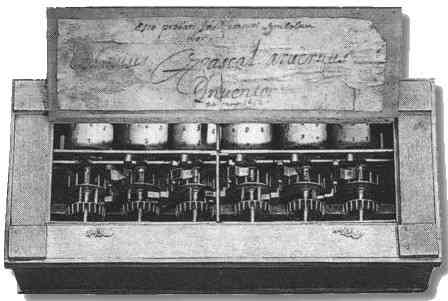
\includegraphics[scale=0.3]{./EtapaPrimeriza/imagenes/cp.jpg}
		\caption{Calculadora Pascalina {\href{https://www.tispain.com/2014/11/la-pascalina-la-primera-calculadora.html}{link}}
\end{figure}
\end{frame}




%%%%%%%%%%%%%%%%%%%%%%%%%%%%%%%%%%%%%%%%%%%%%%%%%%%%%%%%%%%%%%%%%%%%%%%%%%%%%%%%%%%%%%%%%%%%%%
%%                                     LEYES DE LA ROBÓTICA                                 %%
%%%%%%%%%%%%%%%%%%%%%%%%%%%%%%%%%%%%%%%%%%%%%%%%%%%%%%%%%%%%%%%%%%%%%%%%%%%%%%%%%%%%%%%%%%%%%%

\begin{frame}[fragile]{ Isaac Asimov }
\vspace{10px}
\pause
\metroset{block=fill}
\begin{block}{Leyes de la Robótica}
	\begin{enumerate}
		\item Un robot no hará da\~no a un ser humano o, por inacción, permitirá que un ser humano sufra da\~no.
		\pause
		\item Un robot debe cumplir las órdenes dadas por los seres humanos, a excepción de aquellas que entrasen en conflicto con la primera ley
		\pause
		\item Un robot debe proteger su propia existencia en la medida en que esta protección no entre en conflicto con la primera o con la segunda ley
	\end{enumerate}
\end{block}
\end{frame}


%%%%%%%%%%%%%%%%%%%%%%%%%%%%%%%%%%%%%%%%%%%%%%%%%%%%%%%%%%%%%%%%%%%%%%%%%%%%%%%%%%%%%%%%%%%%%%
%%                                TOTUGAS AUTÓNOMAS DE WALTER                               %%
%%%%%%%%%%%%%%%%%%%%%%%%%%%%%%%%%%%%%%%%%%%%%%%%%%%%%%%%%%%%%%%%%%%%%%%%%%%%%%%%%%%%%%%%%%%%%%
\begin{frame}[fragile]{Tortugas Autónomas de Walter}
	\vspace{10px}
	\pause
	\metroset{block=fill}
	\begin{block}{}
		\begin{itemize}
			\item William Grey Walter, Kansas (EE.UU.) en 1910
			\pause
			\item Pionero en el campo de la robótica, cibernética e inteligencia artificial
			\pause
			\item Elmer (1948)
			\pause
			\item Elsie (1948)
		\end{itemize}
	\end{block}
	\begin{figure}
		\centering
		\pause
		\begin{subfigure}{0.48\textwidth}
			\centering
			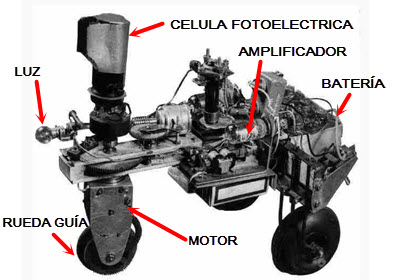
\includegraphics[scale=0.5]{./EtapaPrimeriza/imagenes/t1.jpg}
			\caption{Estructura de las Tortugas Autónomas de Walter {\href{https://vonneumannmachine.files.wordpress.com/2011/05/elsie.jpg}{link}}
		\end{subfigure}
	\end{figure}
\end{frame}

%%%%%%%%%%%%%%%%%%%%%%%%%%%%%%%%%%%%%%%%%%%%%%%%%%%%%%%%%%%%%%%%%%%%%%%%%%%%%%%%%%%%%%%%%%%%%%
%%                              BRAZO ROBÓTICO DE GOERTZ                                    %%
%%%%%%%%%%%%%%%%%%%%%%%%%%%%%%%%%%%%%%%%%%%%%%%%%%%%%%%%%%%%%%%%%%%%%%%%%%%%%%%%%%%%%%%%%%%%%%


\begin{frame}[fragile]{Brazo Robótico de Goertz}
\vspace{10px}
\pause
\metroset{block=fill}
\begin{block}{}
	\begin{itemize}
		\item Raymond Goertz
		\pause
		\item Primer brazo robótico teleoperado
		\pause
		\item Pionero en la técnica maestro-esclavo
	\end{itemize}
\end{block}
\begin{figure}
		\centering
		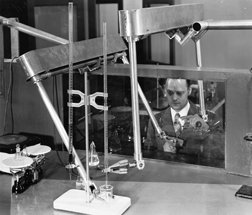
\includegraphics[scale=3.5]{./EtapaPrimeriza/imagenes/brazo.jpg}
		\caption{Brazo Robótico de Goertz {\href{https://en.wikipedia.org/wiki/Raymond\_Goertz\#/media/File:Apf1-06395t.jpg}{link}}
\end{figure}
\end{frame}



%%%%%%%%%%%%%%%%%%%%%%%%%%%%%%%%%%%%%%%%%%%%%%%%%%%%%%%%%%%%%%%%%%%%%%%%%%%%%%%%%%%%%%%%%%%%%%
%%                                        GEORGE DEVOL                                      %%
%%%%%%%%%%%%%%%%%%%%%%%%%%%%%%%%%%%%%%%%%%%%%%%%%%%%%%%%%%%%%%%%%%%%%%%%%%%%%%%%%%%%%%%%%%%%%%

\begin{frame}[fragile]{George Devol}
\vspace{10px}
\pause
\metroset{block=fill}
\begin{block}{}
	\begin{itemize}
		\item Primer robot Industrial en 1948
		\pause
		\item  Joseph F. Engelberger
		\pause
		\item Unimation: Primera empresa robótica de la historia
		\pause 
		\item Generals Motors instala dicho robots en 1960
		\pause
		\item PUMA: \textit{Programmable Universal Machine for Assembly}
	\end{itemize}
\end{block}
\end{frame}


%%%%%%%%%%%%%%%%%%%%%%%%%%%%%%%%%%%%%%%%%%%%%%%%%%%%%%%%%%%%%%%%%%%%%%%%%%%%%%%%%%%%%%%%%%%%%%
%%                                          SPUTNIK                                         %%
%%%%%%%%%%%%%%%%%%%%%%%%%%%%%%%%%%%%%%%%%%%%%%%%%%%%%%%%%%%%%%%%%%%%%%%%%%%%%%%%%%%%%%%%%%%%%%


\begin{frame}[fragile]{Sputnik}
\vspace{10px}
\pause
\metroset{block=fill}
\begin{block}{}
	\begin{itemize}
		\item Programa Sputnik
		\pause
		\item 10 satélites diferentes
	\end{itemize}
\end{block}
\begin{figure}
		\centering
		\pause
		\begin{subfigure}{0.33\textwidth}
			\centering
			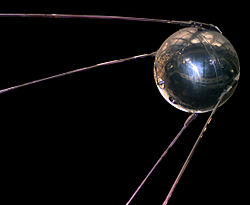
\includegraphics[scale=1.3]{./EtapaPrimeriza/imagenes/s1.jpg}
			\caption{Sputnik 1 {\href{https://es.wikipedia.org/wiki/Sputnik\_1\#/media/File:Sputnik\_asm.jpg}{link}}
		\end{subfigure}
		\pause
		\begin{subfigure}{0.33\textwidth}
			\centering
			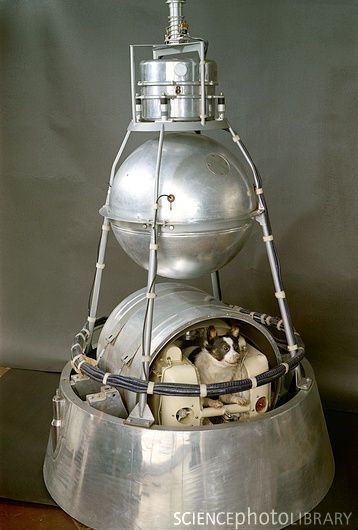
\includegraphics[scale=1.0]{./EtapaPrimeriza/imagenes/s2.jpg}
			\caption{Sputnik 2 {\href{http://www.alas-rojas.com/1-2.htm}{link}}
		\end{subfigure}
		\pause
		\begin{subfigure}{0.32\textwidth}
			\centering
			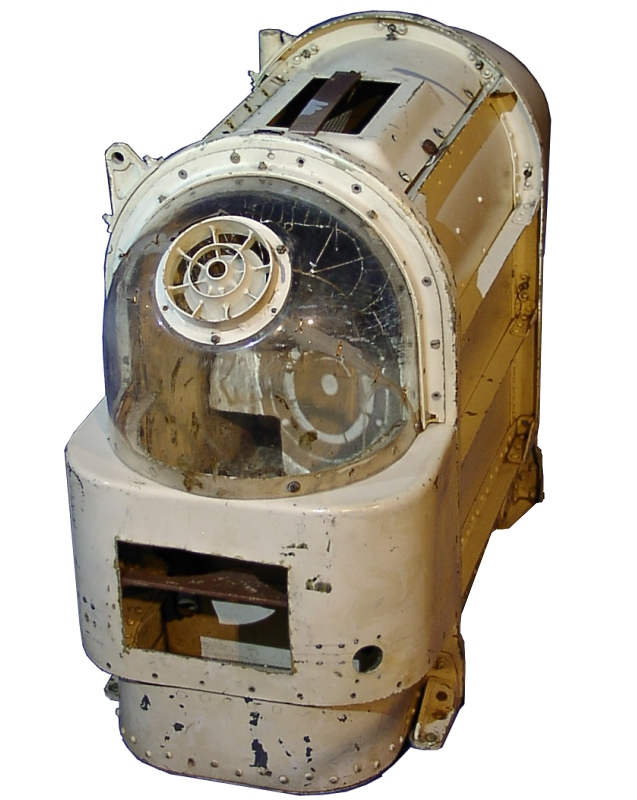
\includegraphics[scale=0.4]{./EtapaPrimeriza/imagenes/s10.jpg}
			\caption{Sputnik 3 {\href{https://es.wikipedia.org/wiki/Sputnik\_10\#/media/File:Russian\_space\_dog\_box.jpg}{link}}
		\end{subfigure}
	\end{figure}
\end{frame}



\section{Etapa Moderna}
%%%%%%%%%%%%%%%%%%%%%%%%%%%%%%%%%%%%%%%%%%%%%%%%%%%%%%%%%%%%%%%%%%%%%%%%%%%%%%%%%%%%%%%%%%%%%%
%%                                      Inicios de la IA                                    %%
%%%%%%%%%%%%%%%%%%%%%%%%%%%%%%%%%%%%%%%%%%%%%%%%%%%%%%%%%%%%%%%%%%%%%%%%%%%%%%%%%%%%%%%%%%%%%%

\begin{frame}[fragile]{Inicios IA}
	\vspace{10px}
	\pause
	\metroset{block=fill}
	\begin{block}{Laboratorios de IA}
		\begin{itemize}
			\item SRI: Shakey, A*, ARPANET.
			\pause
			\item Laboratorio de IA del MIT: McCarthy (Lisp) y Stallman.
			\pause
			\item Robotics Institute: Sandstorm y Highlander.
		\end{itemize}
	\end{block}
	\begin{figure}
		\centering
		\pause
		\begin{subfigure}{0.33\textwidth}
			\centering
			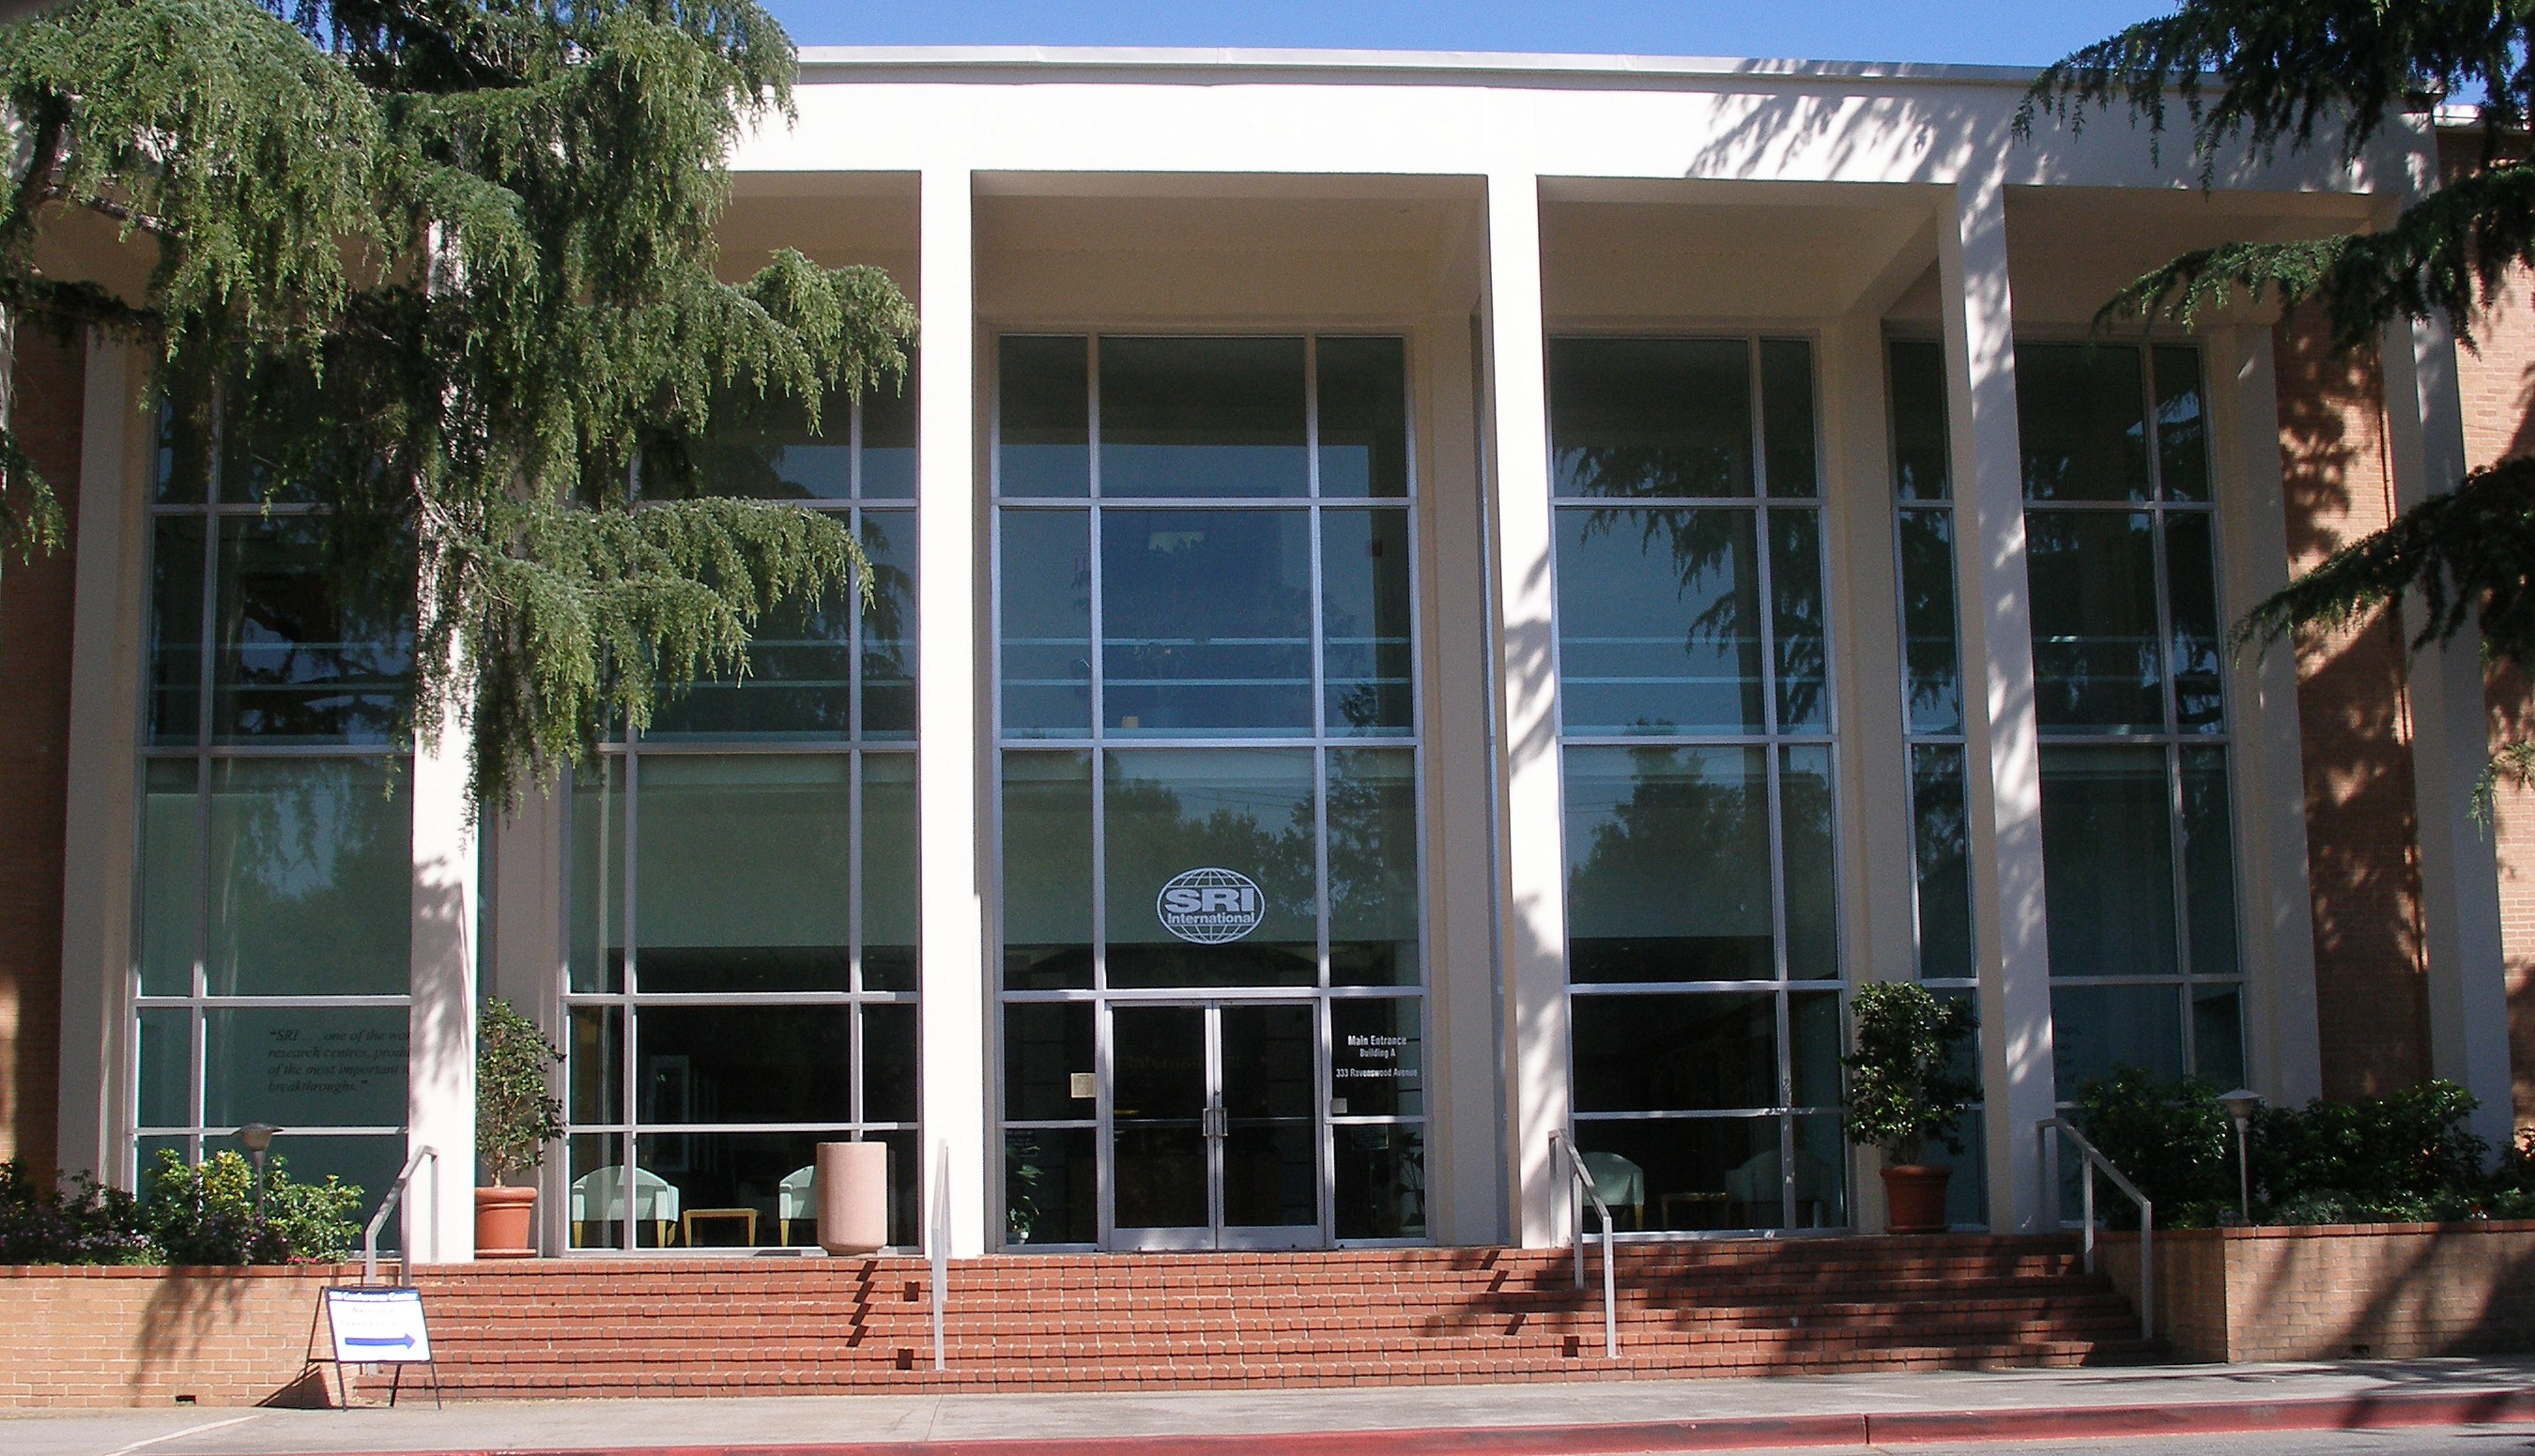
\includegraphics[scale=0.038]{./EtapaModerna/Imagenes/sri.jpg}
			\caption{SRI \href{https://es.m.wikipedia.org/wiki/Archivo:SRI_International_HQ.jpg}{Wikimedia}}
		\end{subfigure}
		\pause
		\begin{subfigure}{0.32\textwidth}
			\centering
			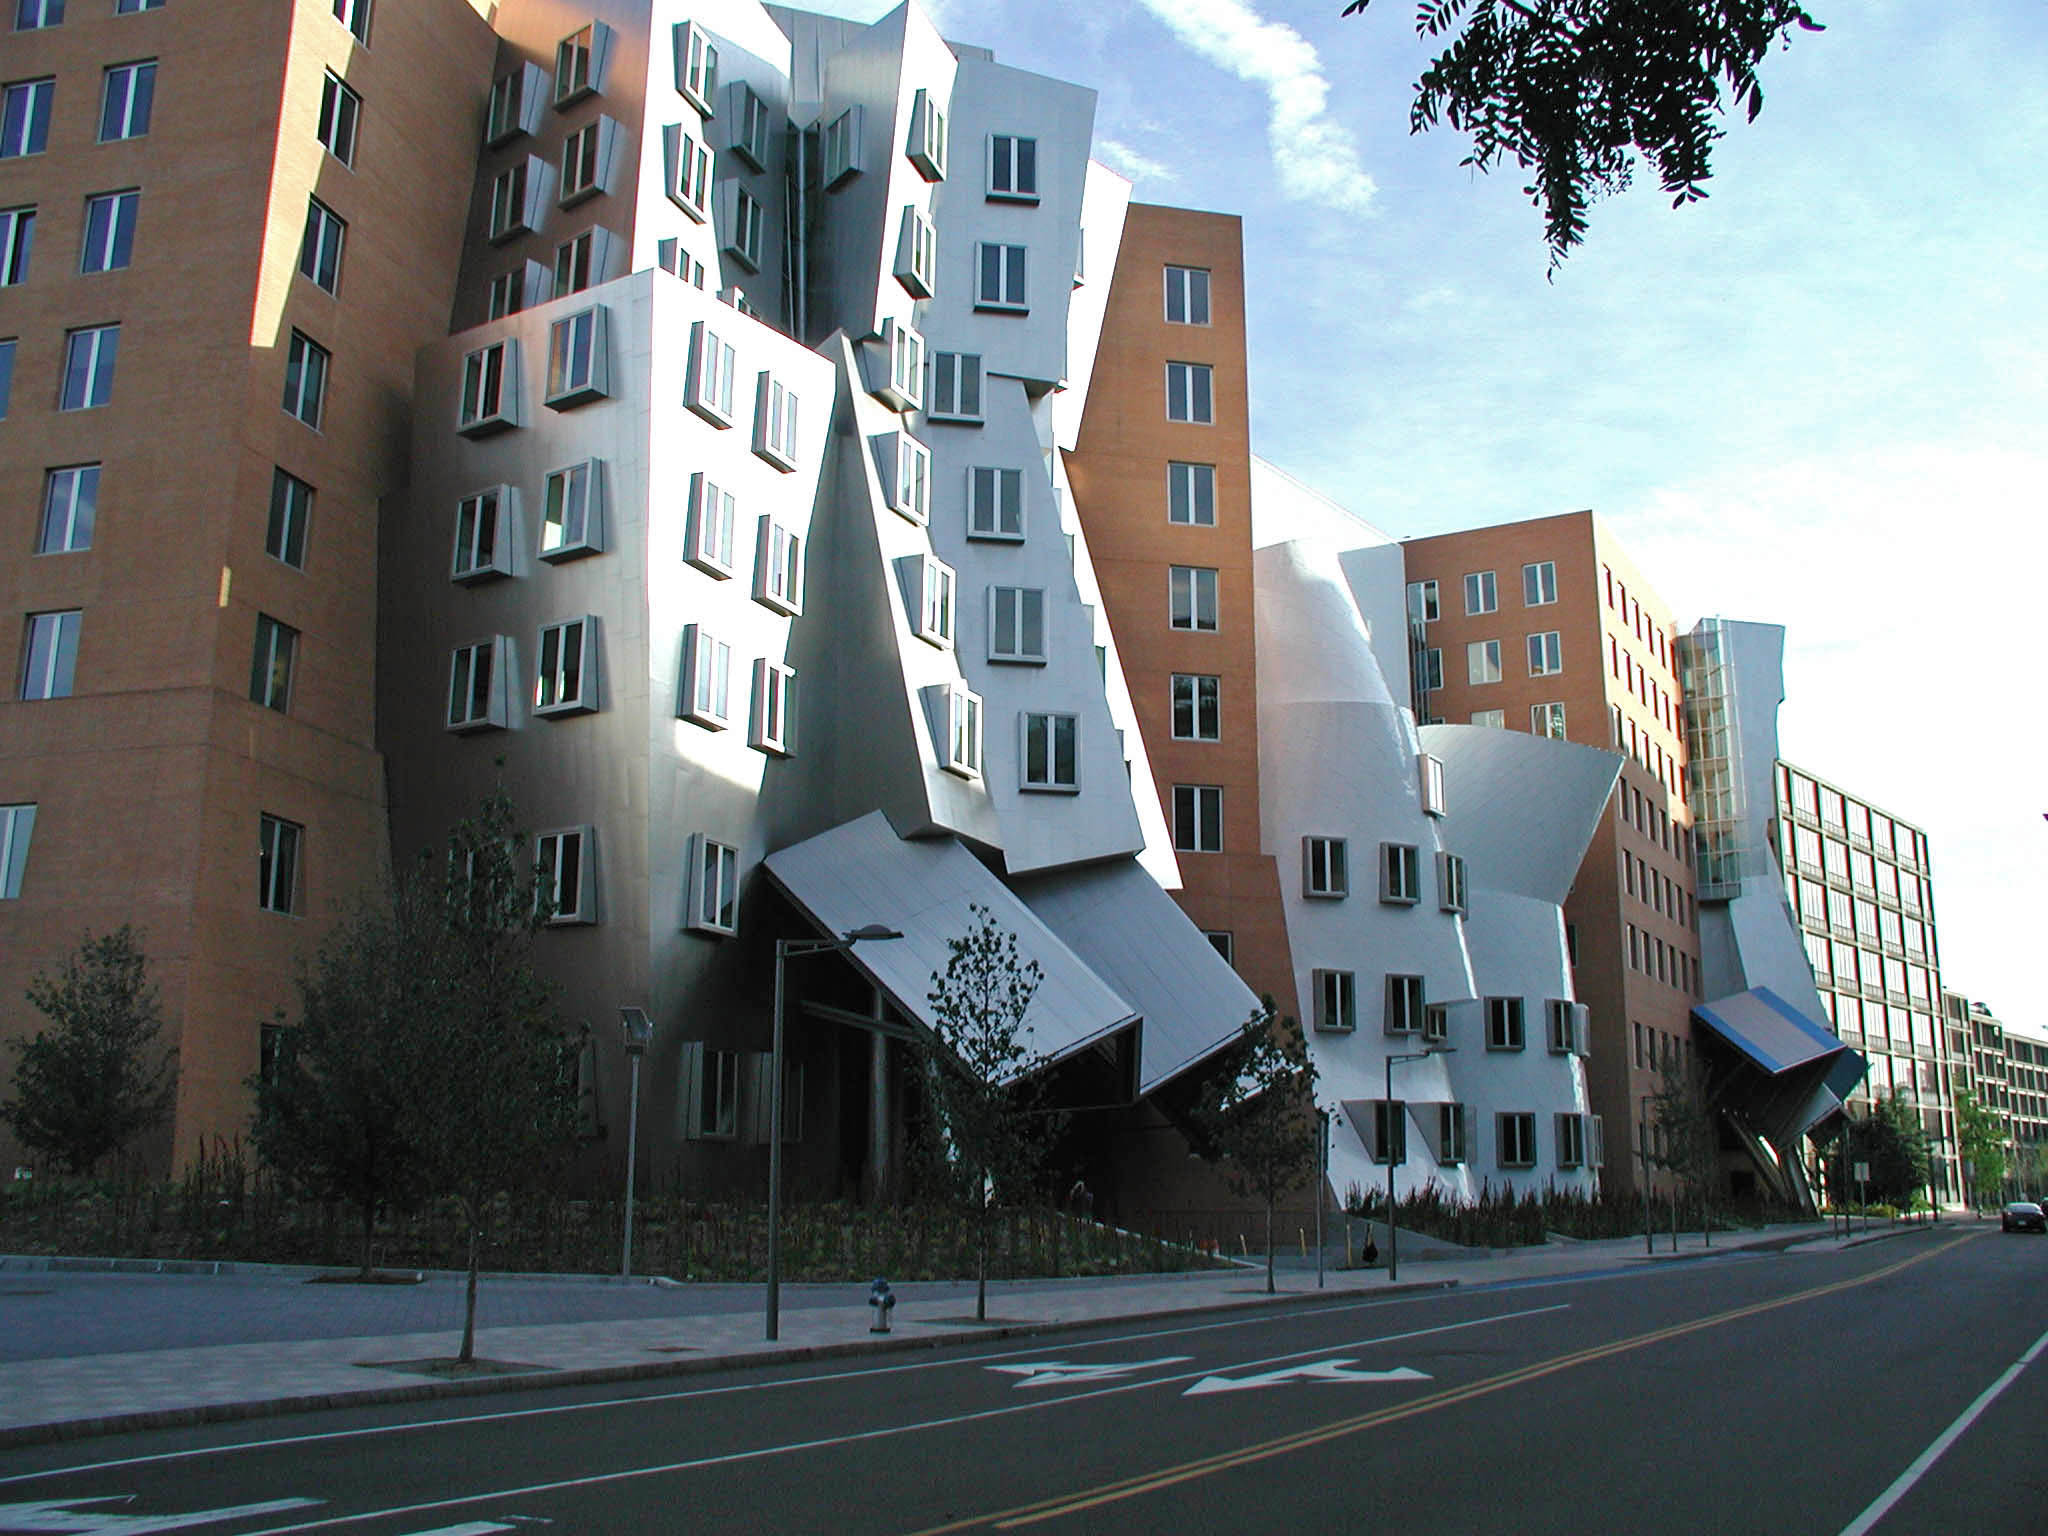
\includegraphics[scale=0.04]{./EtapaModerna/Imagenes/mit_ai.jpg}
			\caption{MIT AI Lab \href{https://commons.wikimedia.org/wiki/File:Stata_Center1.jpg}{Wikimedia}}
		\end{subfigure}
		\pause
		\begin{subfigure}{0.33\textwidth}
			\centering
			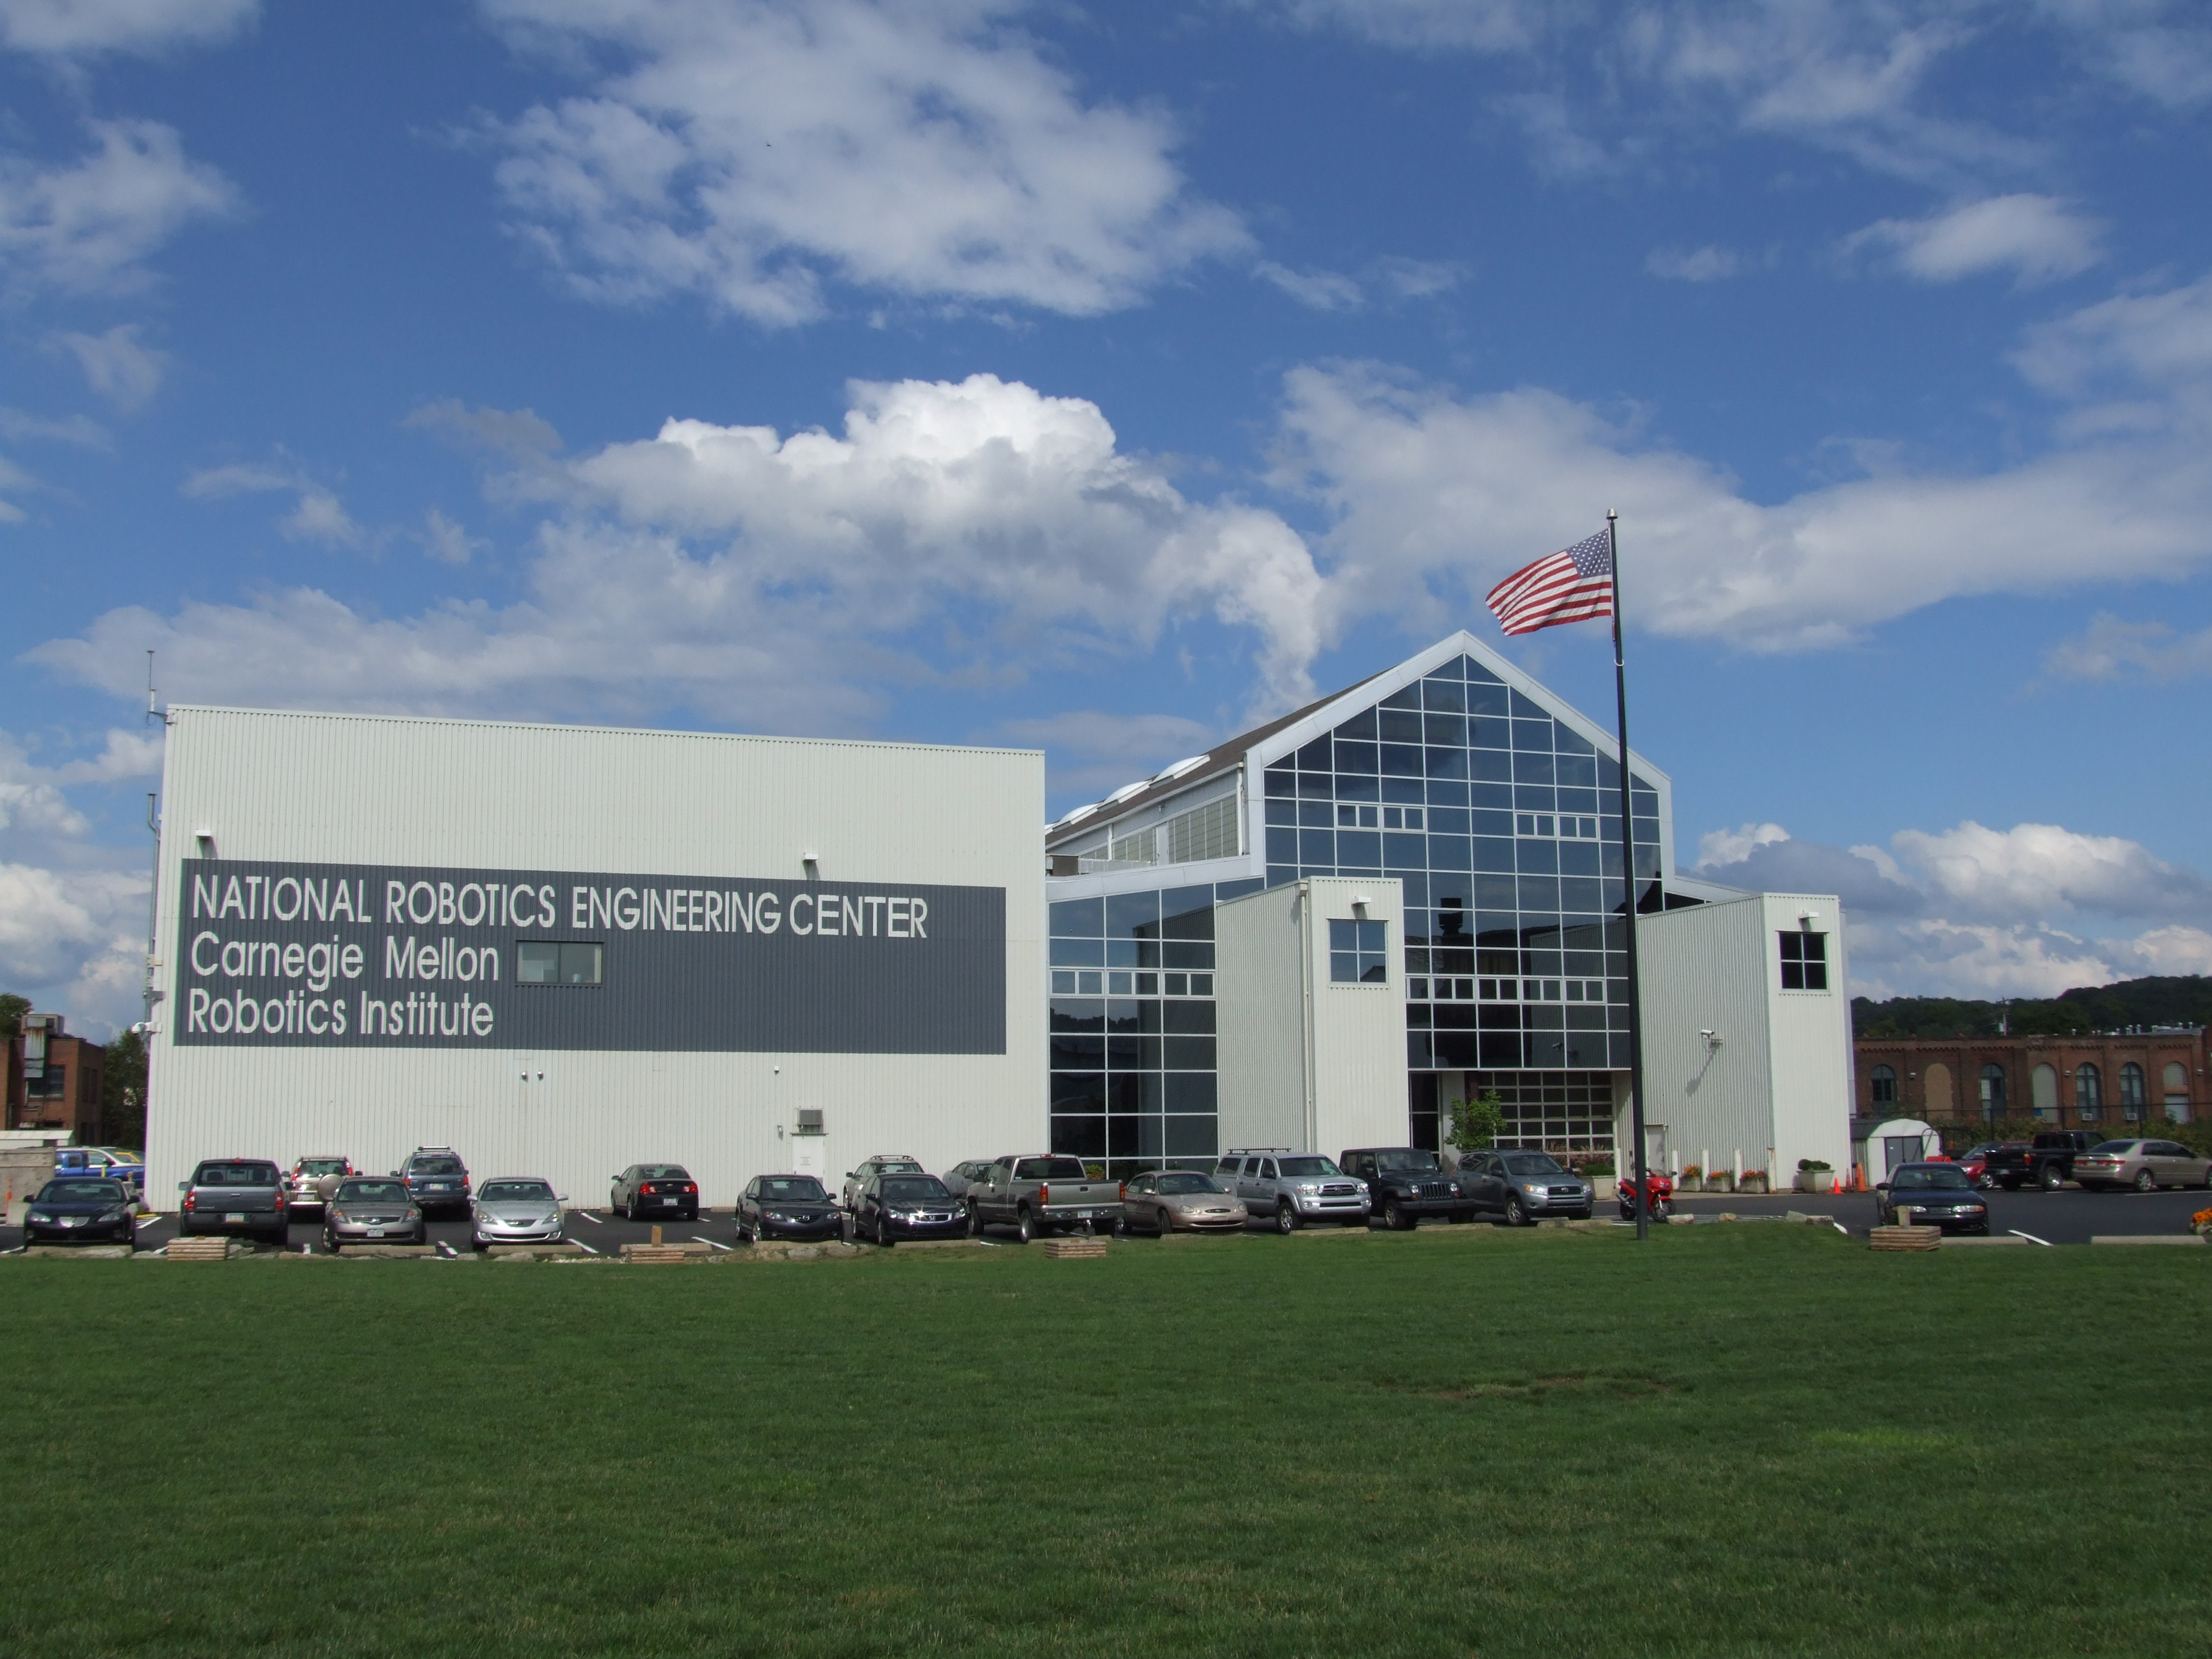
\includegraphics[scale=0.026]{./EtapaModerna/Imagenes/robotics_institute.jpg}
			\caption{Robotics Institute \href{https://commons.wikimedia.org/wiki/File:National_Robotics_Engineering_Center.JPG}{Wikimedia}}
		\end{subfigure}
	\end{figure}
\end{frame}

%%%%%%%%%%%%%%%%%%%%%%%%%%%%%%%%%%%%%%%%%%%%%%%%%%%%%%%%%%%%%%%%%%%%%%%%%%%%%%%%%%%%%%%%%%%%%%
%%                                     Brazos Robóticos                                     %%
%%%%%%%%%%%%%%%%%%%%%%%%%%%%%%%%%%%%%%%%%%%%%%%%%%%%%%%%%%%%%%%%%%%%%%%%%%%%%%%%%%%%%%%%%%%%%%

\begin{frame}[fragile]{Brazos Robóticos}
\vspace{10px}
\pause
\metroset{block=fill}
\begin{block}{Brazos Robóticos}
	\begin{itemize}
		\item Stanford Arm: eléctrico con 6 grados de libertad. \href{https://www.youtube.com/watch?v=r4aNOM3IK7A}{(Vídeo)}
		\pause
		\item PUMA: programable fabricado por General Motors.
		\pause
		\item SCARA: primer brazo con giro en el eje Z.
	\end{itemize}
\end{block}
\begin{figure}
	\centering
	\pause
	\begin{subfigure}{0.33\textwidth}
		\centering
		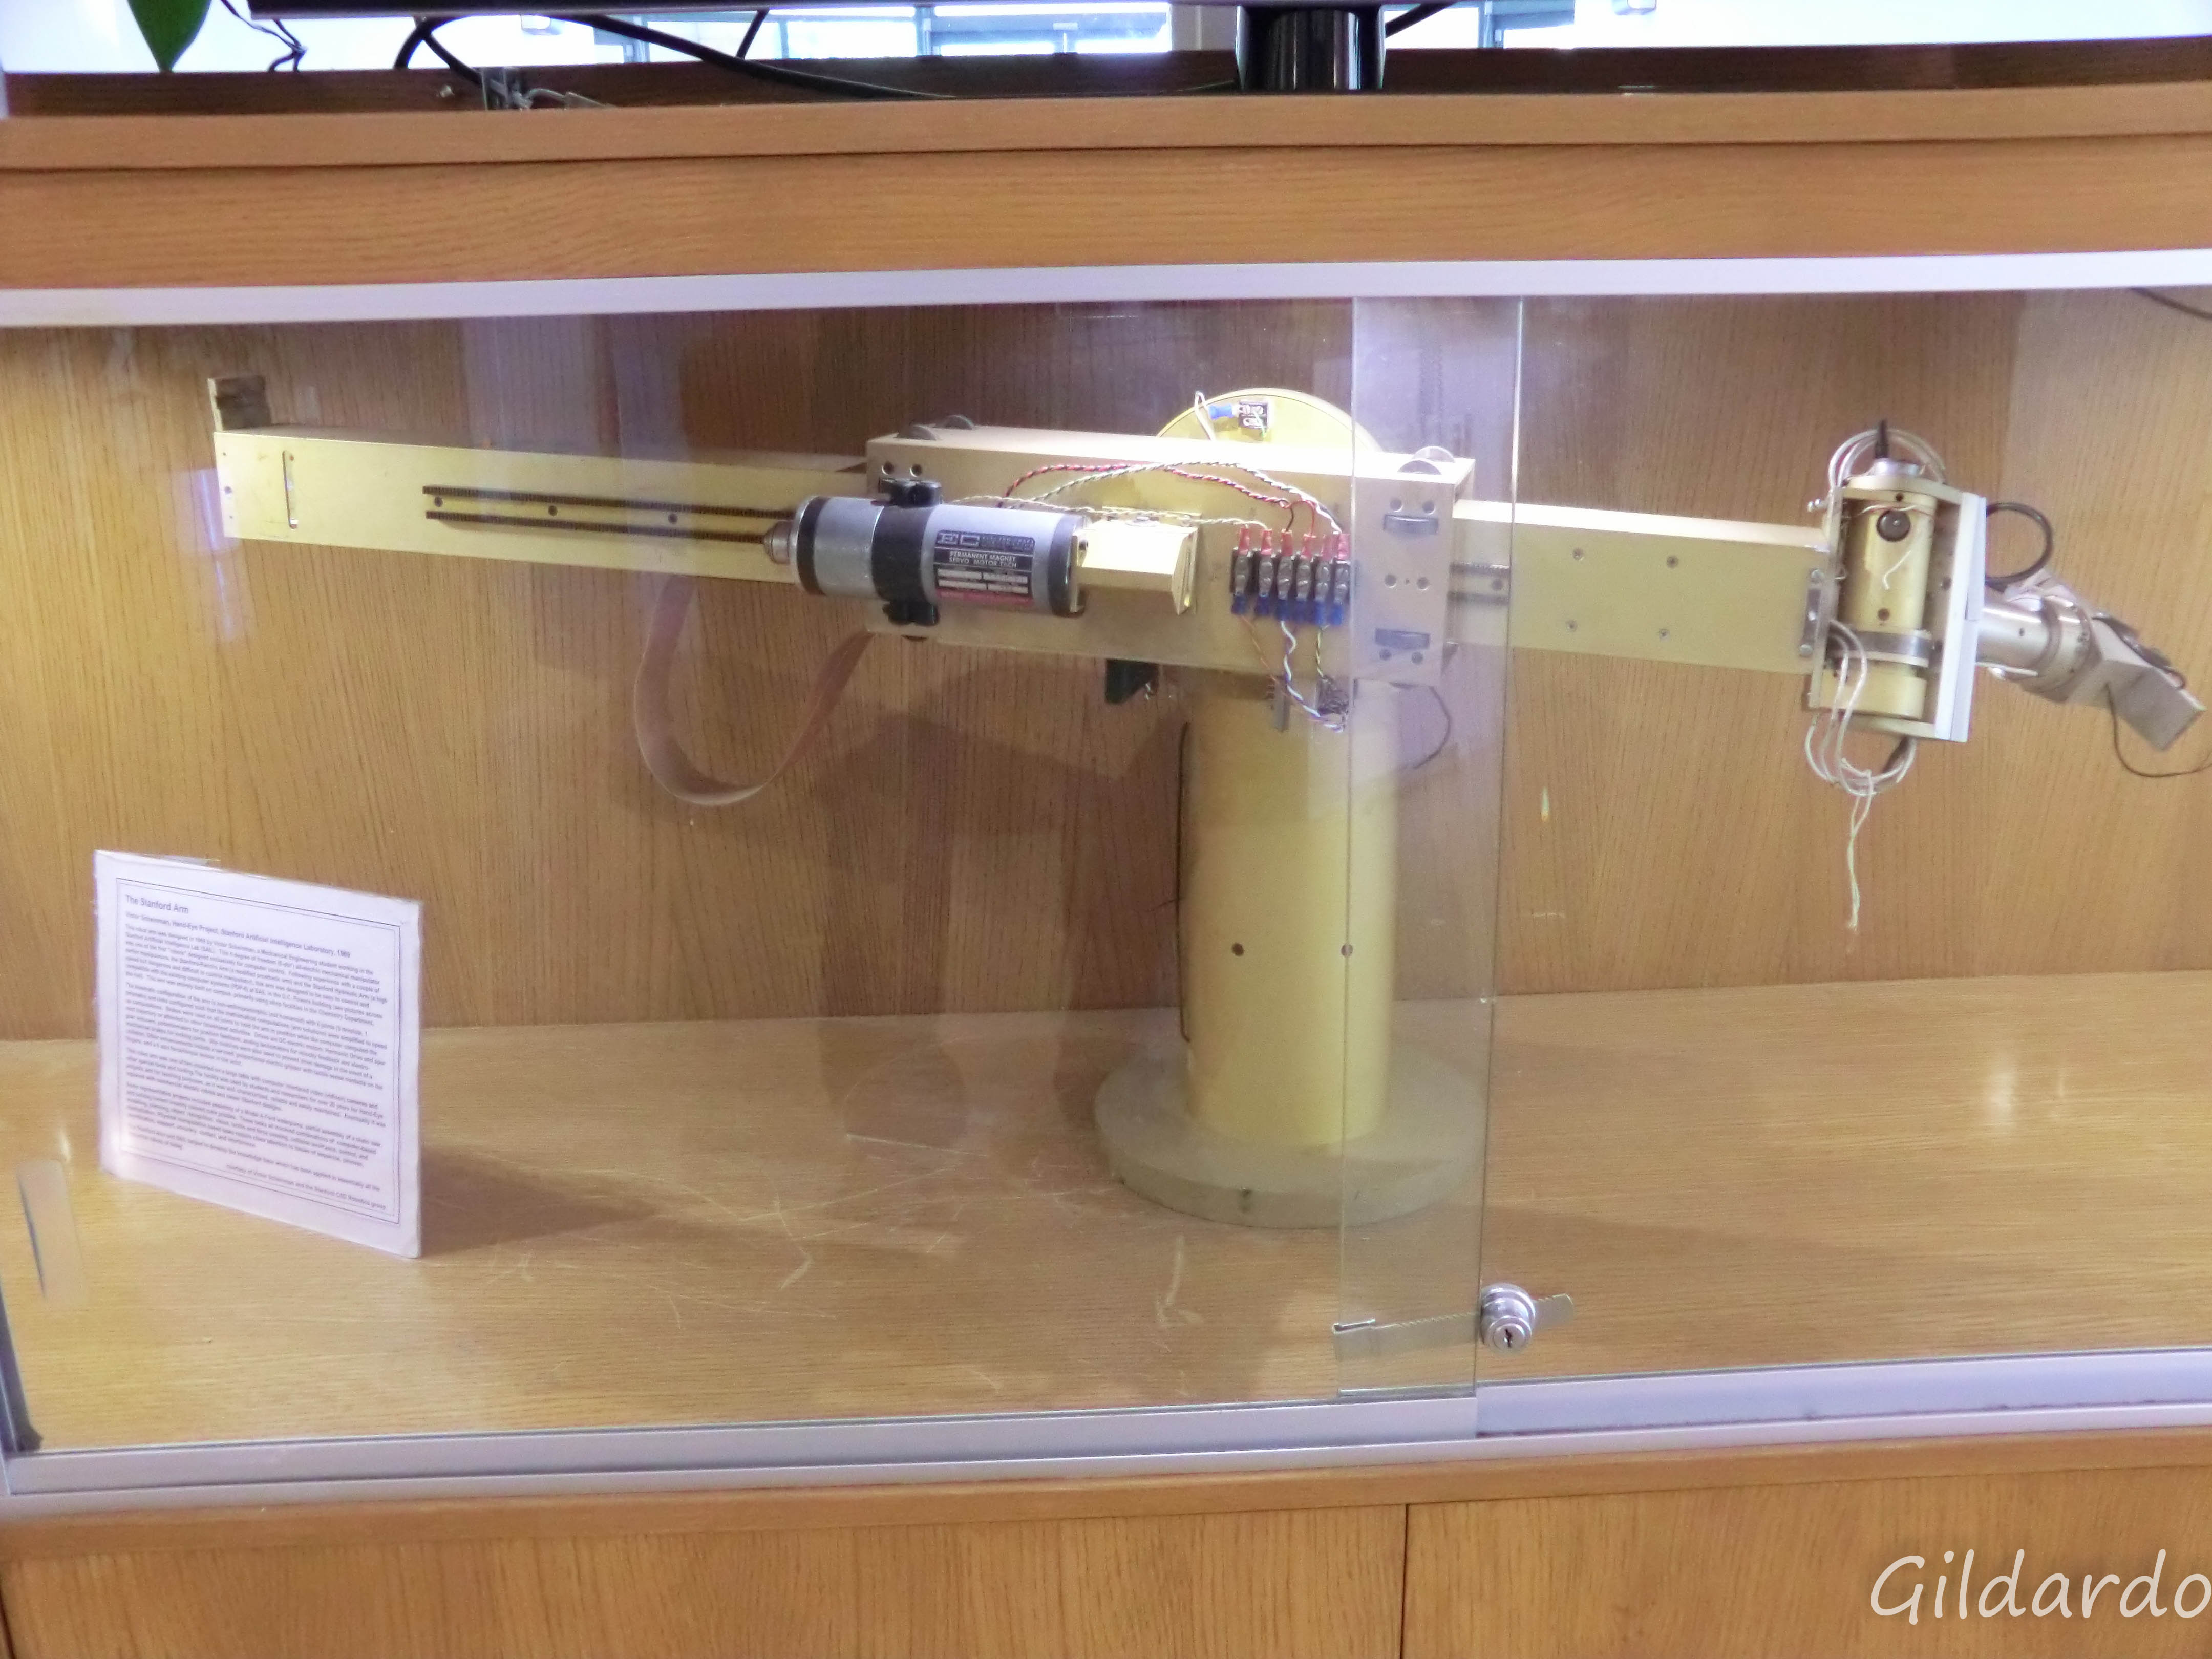
\includegraphics[scale=0.08]{./EtapaModerna/Imagenes/stanford_arm.jpg}
		\caption{Stanford Arm \href{https://www.flickr.com/photos/gildardo/6186967797}{Flickr}}
	\end{subfigure}
	\pause
	\begin{subfigure}{0.32\textwidth}
		\centering
		\includegraphics[scale=0.12]{./EtapaModerna/Imagenes/puma.jpg}
		\caption{PUMA \href{https://es.m.wikipedia.org/wiki/Archivo:Puma_Robotic_Arm_-_GPN-2000-001817.jpg}{Wikimedia}}
	\end{subfigure}
	\pause
	\begin{subfigure}{0.33\textwidth}
		\centering
		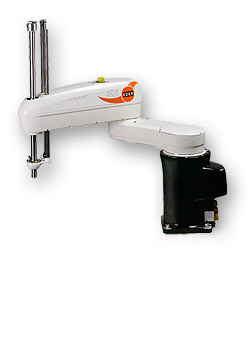
\includegraphics[scale=0.3]{./EtapaModerna/Imagenes/SCARA.jpg}
		\caption{SCARA \href{https://commons.wikimedia.org/wiki/File:KUKA_Industrial_Robot_KR10_SCARA.jpg}{Wikimedia}}
	\end{subfigure}
\end{figure}
\end{frame}

%%%%%%%%%%%%%%%%%%%%%%%%%%%%%%%%%%%%%%%%%%%%%%%%%%%%%%%%%%%%%%%%%%%%%%%%%%%%%%%%%%%%%%%%%%%%%%
%%                                        Movimiento                                        %%
%%%%%%%%%%%%%%%%%%%%%%%%%%%%%%%%%%%%%%%%%%%%%%%%%%%%%%%%%%%%%%%%%%%%%%%%%%%%%%%%%%%%%%%%%%%%%%

\begin{frame}[fragile]{Movimiento}
\vspace{10px}
\pause
\metroset{block=fill}
\begin{block}{Avance en el movimiento}
	\begin{itemize}
		\item Antecesores: RB5X, Phony Pony, WAP, Aquarobot, ...
		\pause
		\item ASIMO: \href{https://www.youtube.com/watch?v=mI58DU1hu14}{(Vídeo)}
	\end{itemize}
\end{block}
\begin{figure}
	\centering
	\pause
	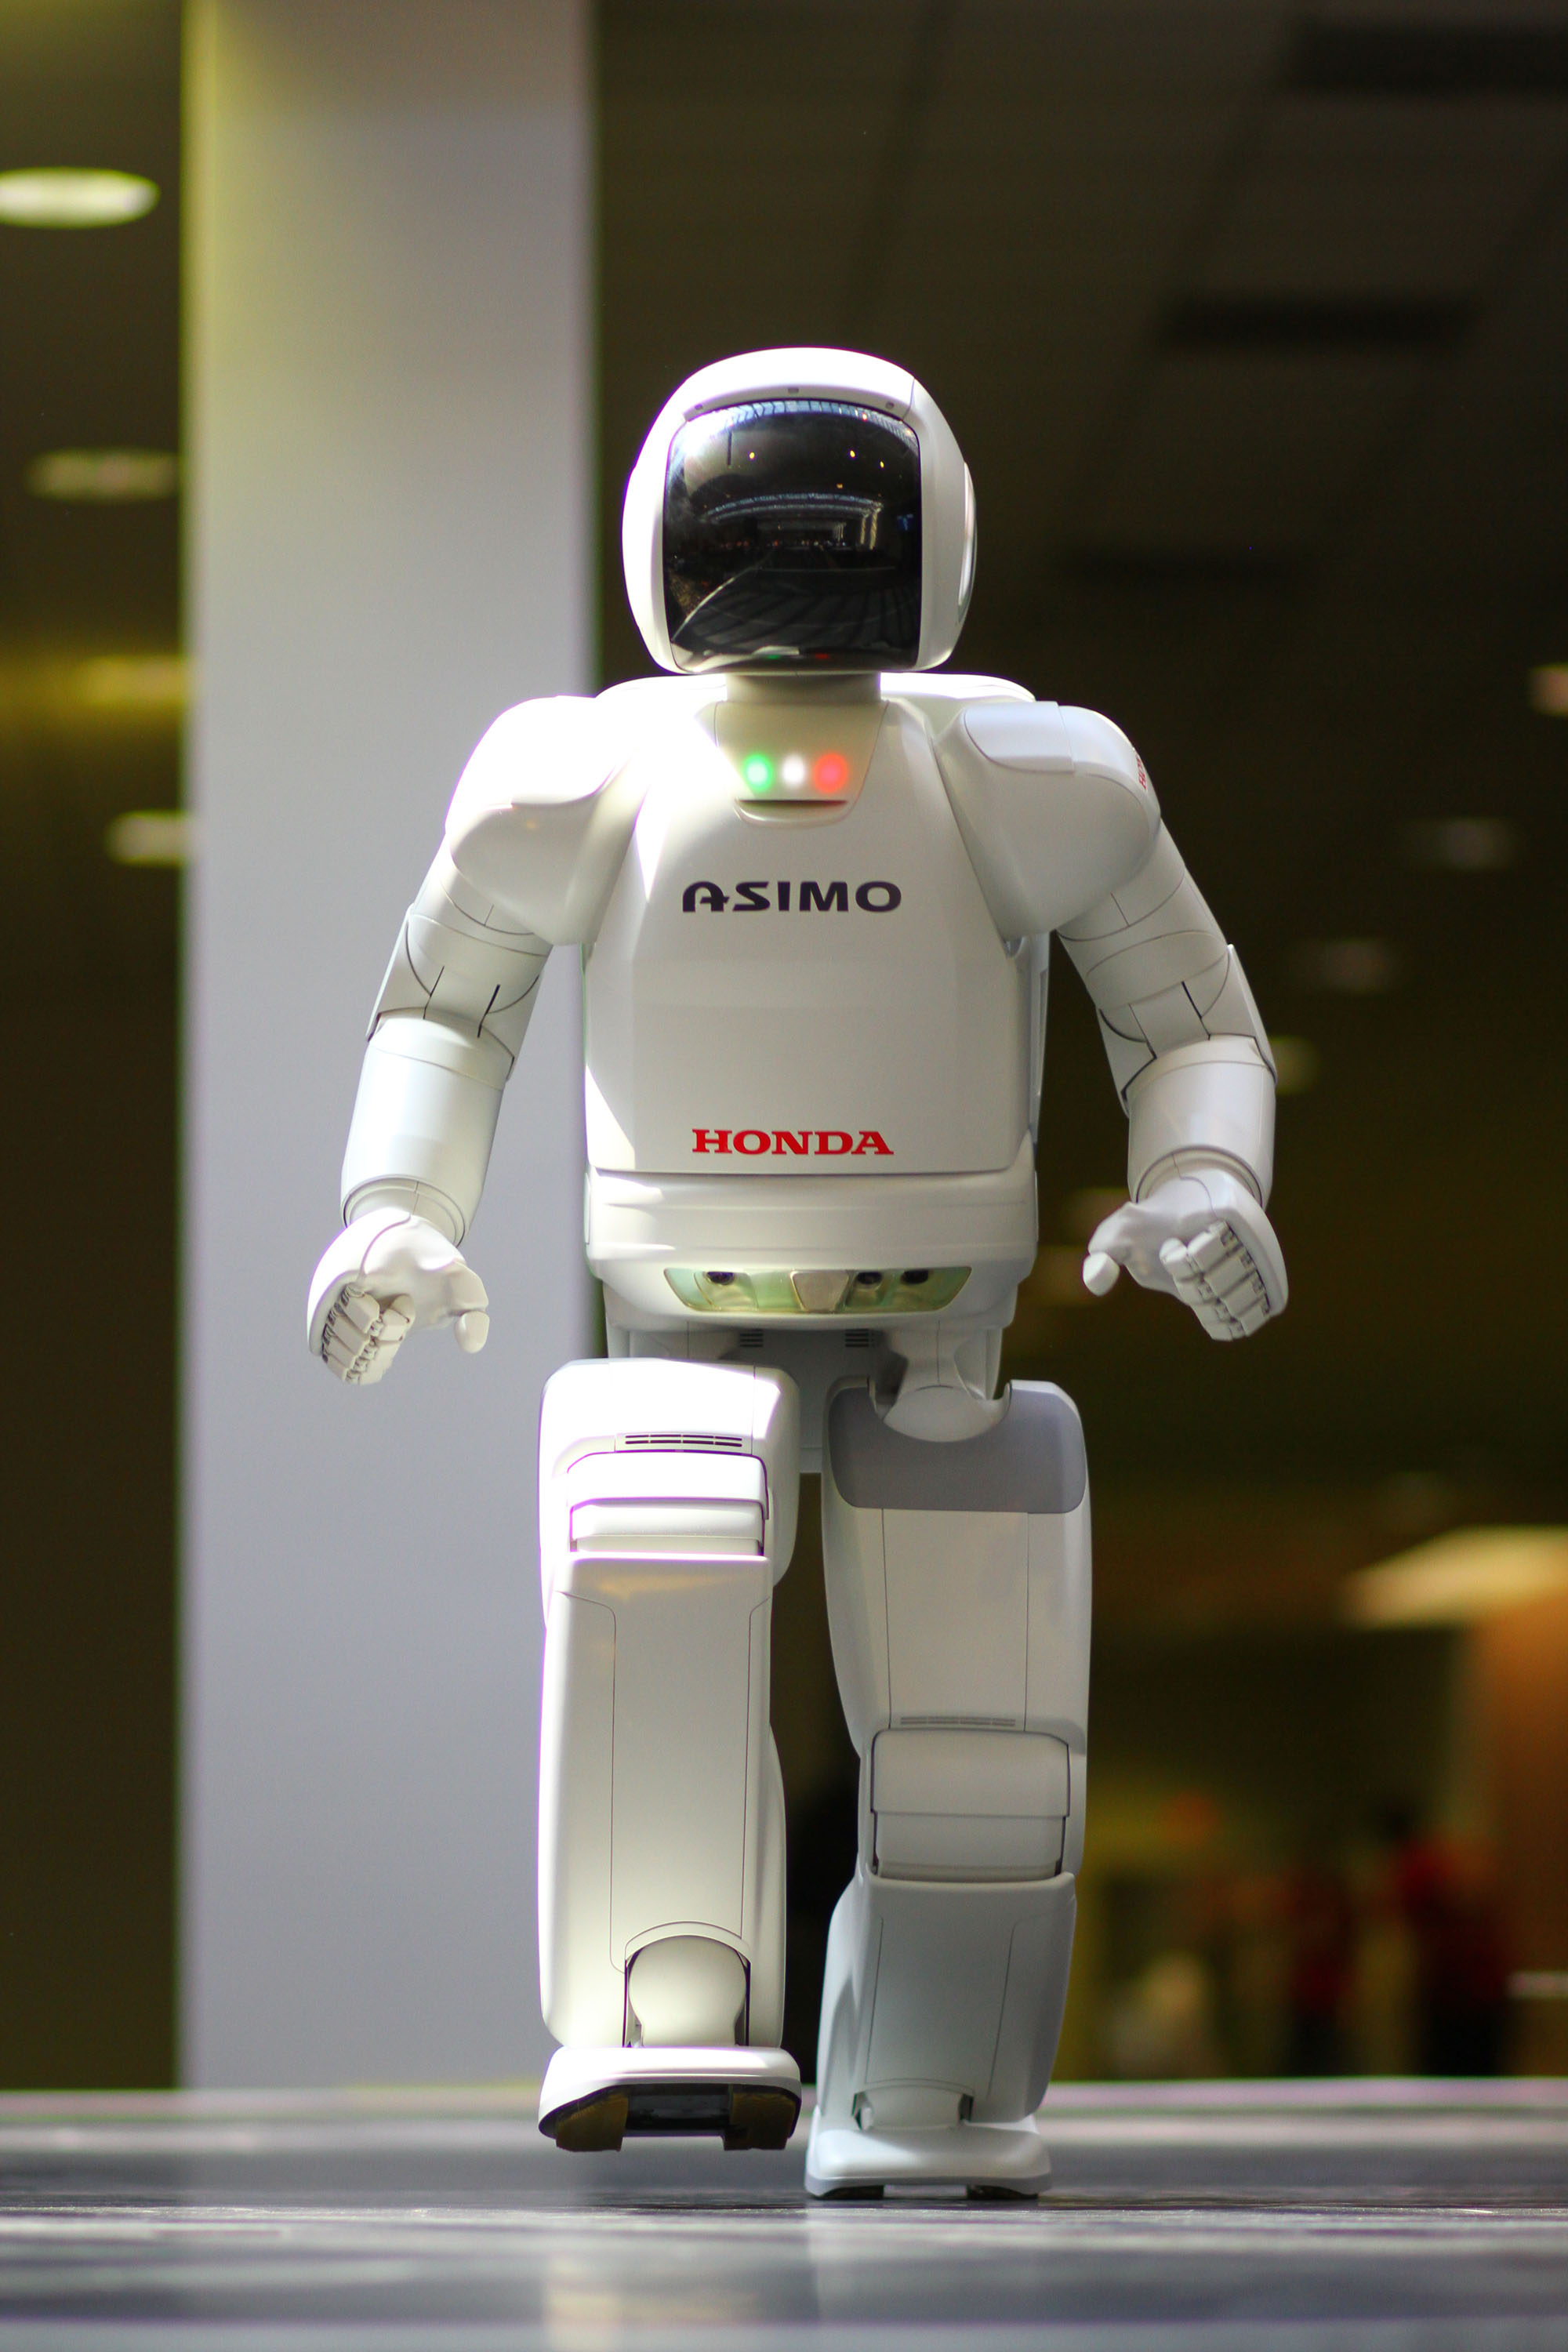
\includegraphics[scale=0.12]{./EtapaModerna/Imagenes/asimo.jpg}
	\caption{ASIMO \href{https://es.m.wikipedia.org/wiki/Archivo:ASIMO_4.28.11.jpg}{Wikimedia}}
\end{figure}
\end{frame}

%%%%%%%%%%%%%%%%%%%%%%%%%%%%%%%%%%%%%%%%%%%%%%%%%%%%%%%%%%%%%%%%%%%%%%%%%%%%%%%%%%%%%%%%%%%%%%
%%                                     Estado del Arte                                      %%
%%%%%%%%%%%%%%%%%%%%%%%%%%%%%%%%%%%%%%%%%%%%%%%%%%%%%%%%%%%%%%%%%%%%%%%%%%%%%%%%%%%%%%%%%%%%%%

\begin{frame}[fragile]{Estado del Arte}
\vspace{10px}
\pause
\metroset{block=fill}
\begin{block}{Principales Campos}
	\begin{itemize}
		\item NASA
		\pause
		\item Robots militares
		\pause
		\item Inteligencia Artificial
		\pause
		\item Robots Humanoides
	\end{itemize}
\end{block}
\end{frame}

%%%%%%%%%%%%%%%%%%%%%%%%%%%%%%%%%%%%%%%%%%%%%%%%%%%%%%%%%%%%%%%%%%%%%%%%%%%%%%%%%%%%%%%%%%%%%%
%%                                           NASA                                           %%
%%%%%%%%%%%%%%%%%%%%%%%%%%%%%%%%%%%%%%%%%%%%%%%%%%%%%%%%%%%%%%%%%%%%%%%%%%%%%%%%%%%%%%%%%%%%%%

\begin{frame}[fragile]{NASA}
\vspace{10px}
\pause
\metroset{block=fill}
\begin{block}{Brazos Robóticos}
	\begin{itemize}
		\item Robonaut \href{https://www.youtube.com/watch?v=JLU0c0mmvxg}{(Vídeo)}, Dextre \href{https://www.youtube.com/watch?v=AXQ6iSFVwrk}{(Vídeo)}, Rassor \href{https://www.youtube.com/watch?v=d3zRvl2LYJ4}{(Vídeo)}
		\pause
		\item InSight \href{https://www.youtube.com/watch?v=LKLITDmm4NA}{(Vídeo)} y Mars 2020 \href{https://www.youtube.com/watch?v=iZCRFRgSgas&t=327s}{(Vídeo)}
		\pause
		\item Curiosity \href{https://www.youtube.com/watch?v=P4boyXQuUIw}{(Vídeo)}
	\end{itemize}
\end{block}
\begin{figure}
	\centering
	\pause
	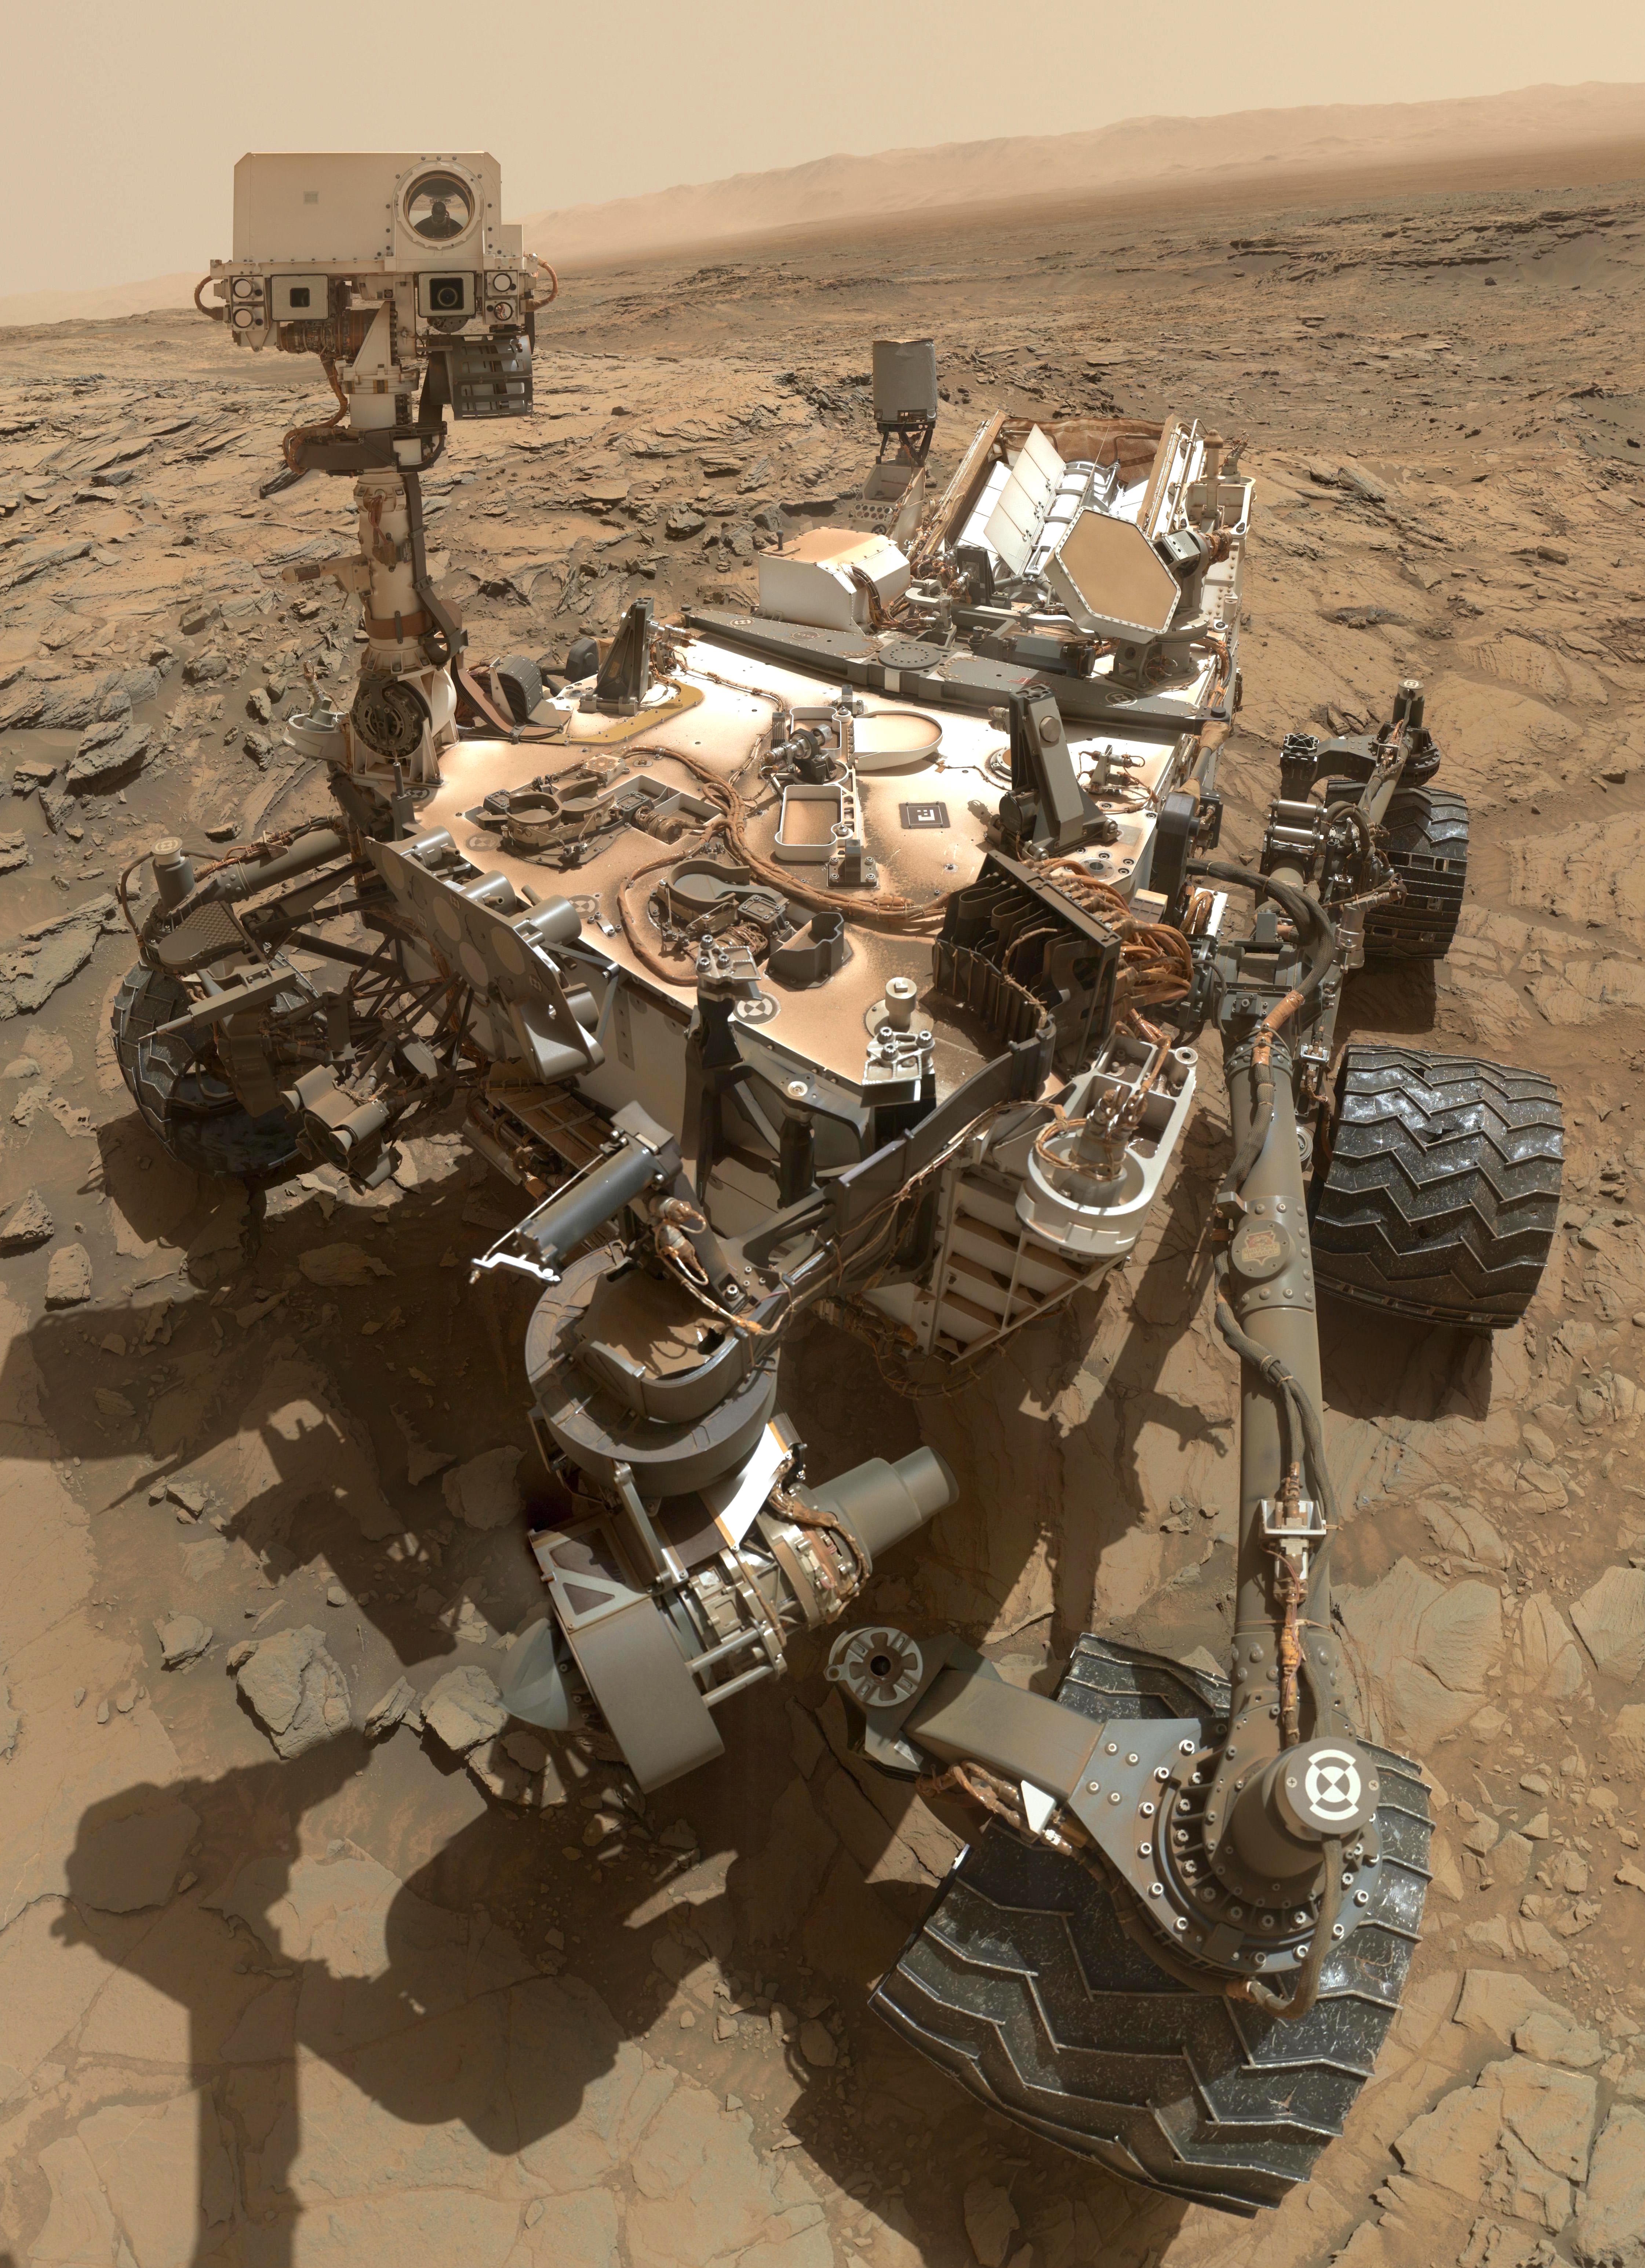
\includegraphics[scale=0.019]{./EtapaModerna/Imagenes/curiosity.jpg}
	\caption{Curiosity \href{https://en.wikipedia.org/wiki/File:Curiosity_Self-Portrait_at_\%27Big_Sky\%27_Drilling_Site.jpg}{Wikimedia}}
\end{figure}
\end{frame}

%%%%%%%%%%%%%%%%%%%%%%%%%%%%%%%%%%%%%%%%%%%%%%%%%%%%%%%%%%%%%%%%%%%%%%%%%%%%%%%%%%%%%%%%%%%%%%
%%                                     Robots militares                                     %%
%%%%%%%%%%%%%%%%%%%%%%%%%%%%%%%%%%%%%%%%%%%%%%%%%%%%%%%%%%%%%%%%%%%%%%%%%%%%%%%%%%%%%%%%%%%%%%

\begin{frame}[fragile]{Robots Militares}
\vspace{10px}
\pause
\metroset{block=fill}
\begin{block}{Robots Militares}
	\begin{itemize}
		\item Elbit Hermes 450 \href{https://www.youtube.com/watch?v=hpa9MkE58sM}{(Vídeo)}
		\pause
		\item Guardium \href{https://www.youtube.com/watch?v=ESS5lW_Os2Q}{(Vídeo)}
		\pause
		\item TALON \href{https://www.youtube.com/watch?v=kDtucLAXpm4}{(Vídeo)}
		\pause
		\item SGR-A1 \href{https://www.youtube.com/watch?v=azQzwI9-GHU}{(Vídeo)}
	\end{itemize}
\end{block}
\begin{figure}
	\centering
	\pause
	\centering
	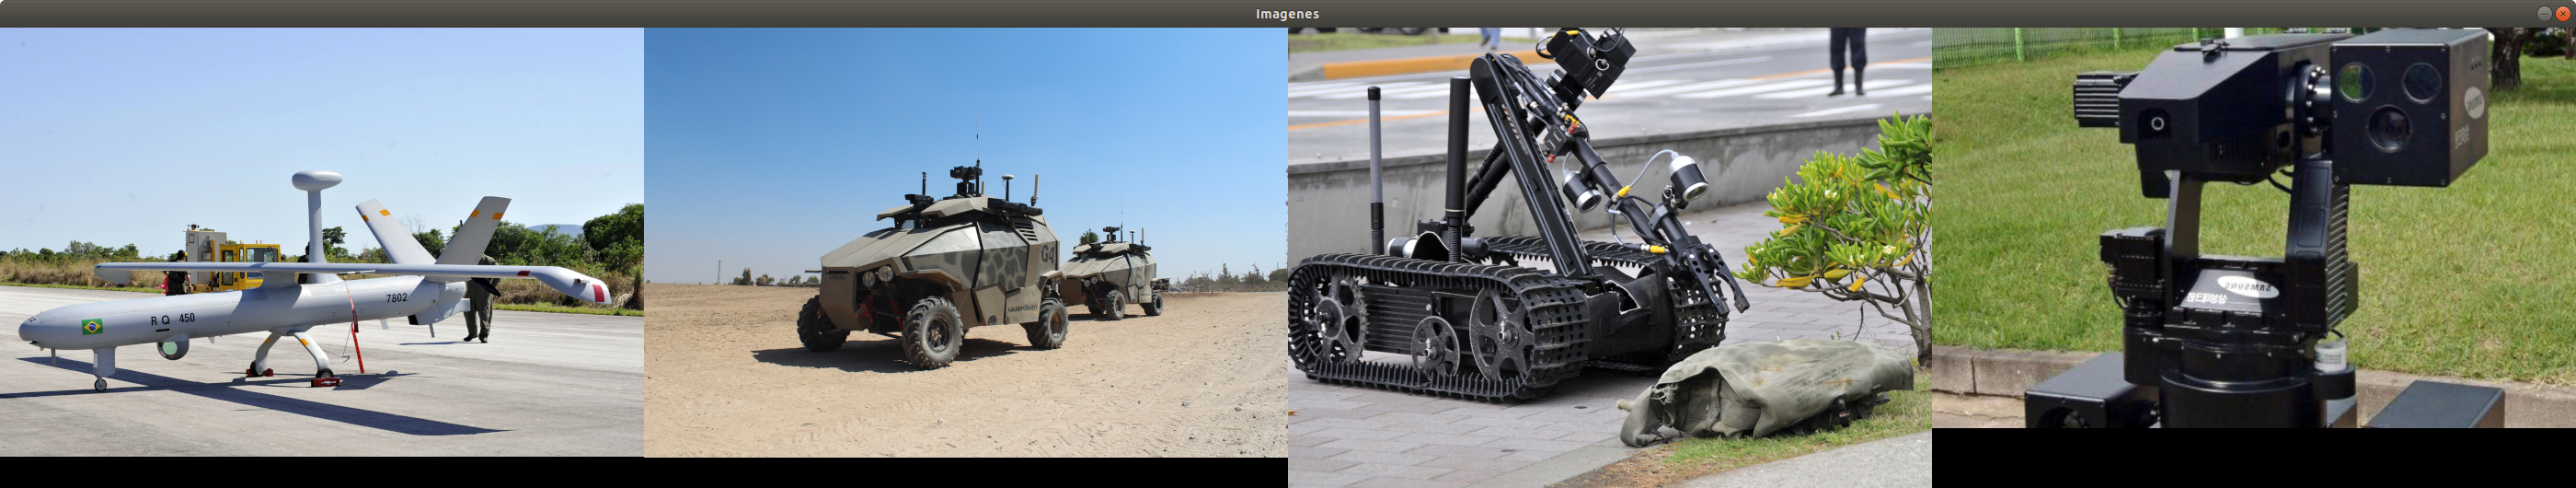
\includegraphics[scale=0.11]{./EtapaModerna/Imagenes/robots_militares.png}
	\caption{Elbit Hermes 450 \href{https://commons.wikimedia.org/wiki/File:Vant_Hermes_450_da_FAB_no_aeroporto_de_C\%C3\%A1ceres_(MT)_(8101398607).jpg}{Wikimedia}, Guardium \href{https://ca.wikipedia.org/wiki/Fitxer:Flickr_-_Israel_Defense_Forces_-_Israeli_Made_Guardium_UGV_(5).jpg}{Wikimedia}, TALON \href{https://commons.wikimedia.org/wiki/File:US_Navy_090512-N-2013O-013_A_Mark_II_Talon_robot_from_Explosive_Ordnance_Disposal_Mobile_Unit_5,_Det._Japan,_is_used_to_inspect_a_suspicious_package_during_a_force_protection-anti-terrorism_training_exercise.jpg}{Wikimedia}, SGR-A1 \href{https://commons.wikimedia.org/wiki/File:SGR-A1.jpg}{Wikimedia}}
\end{figure}
\end{frame}

%%%%%%%%%%%%%%%%%%%%%%%%%%%%%%%%%%%%%%%%%%%%%%%%%%%%%%%%%%%%%%%%%%%%%%%%%%%%%%%%%%%%%%%%%%%%%%
%%                                        Avances IA                                        %%
%%%%%%%%%%%%%%%%%%%%%%%%%%%%%%%%%%%%%%%%%%%%%%%%%%%%%%%%%%%%%%%%%%%%%%%%%%%%%%%%%%%%%%%%%%%%%%

\begin{frame}[fragile]{Avances de la IA}
\vspace{10px}
\pause
\metroset{block=fill}
\begin{block}{Sectores principales}
	\begin{itemize}
		\item Salud: Watson, brazos robóticos, prótesis, ... \href{https://www.youtube.com/watch?v=0XdC1HUp-rU}{(Vídeo Sutura Uva)}
		\pause
		\item Automoción: conducción inteligente y asistencia. \href{https://www.youtube.com/watch?v=IkSw2SZQENU}{(Vídeo Autopilot)}
		\pause
		\item Economía: análisis de la banca y operaciones en bolsa.
		\pause
		\item Publicidad: más efectiva.
	\end{itemize}
\end{block}
\begin{figure}
	\centering
	\pause
	\begin{subfigure}{0.45\textwidth}
		\centering
		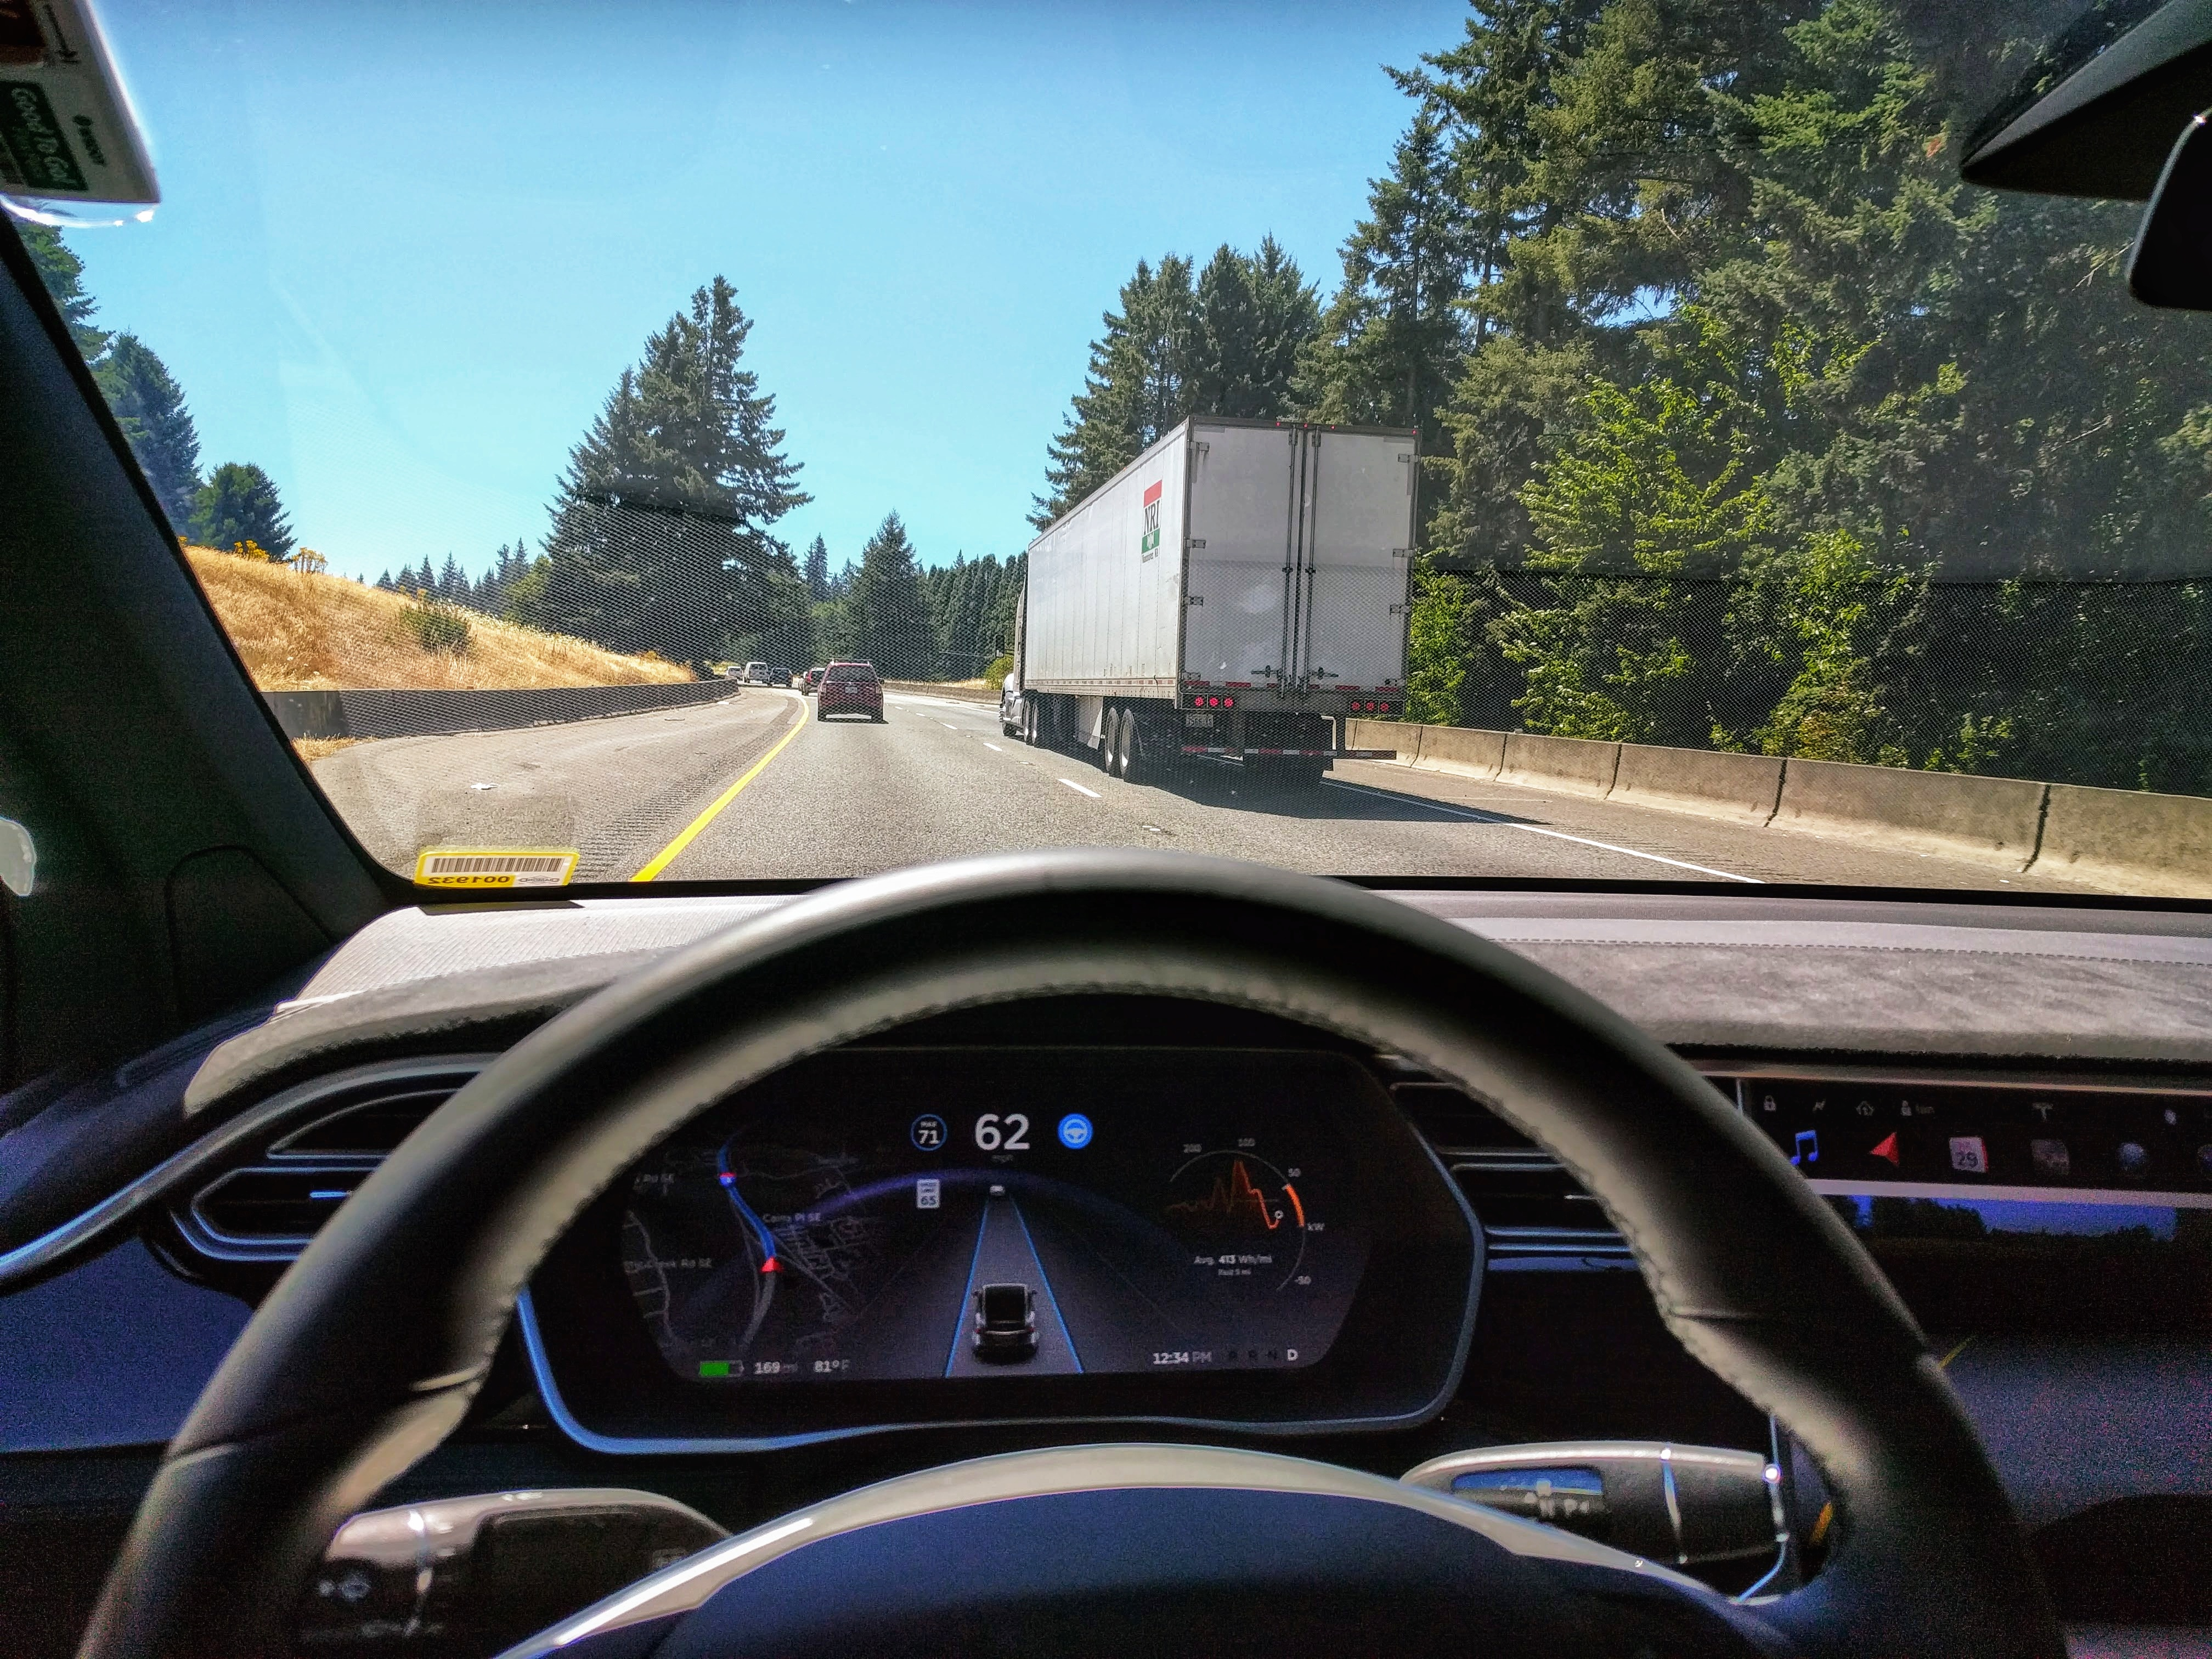
\includegraphics[scale=0.025]{./EtapaModerna/Imagenes/autopilot.jpg}
		\caption{Autopilot \href{https://commons.wikimedia.org/wiki/File:Tesla_Autopilot_Engaged_in_Model_X.jpg}{Wikimedia}}
	\end{subfigure}
	\pause
	\begin{subfigure}{0.45\textwidth}
		\centering
		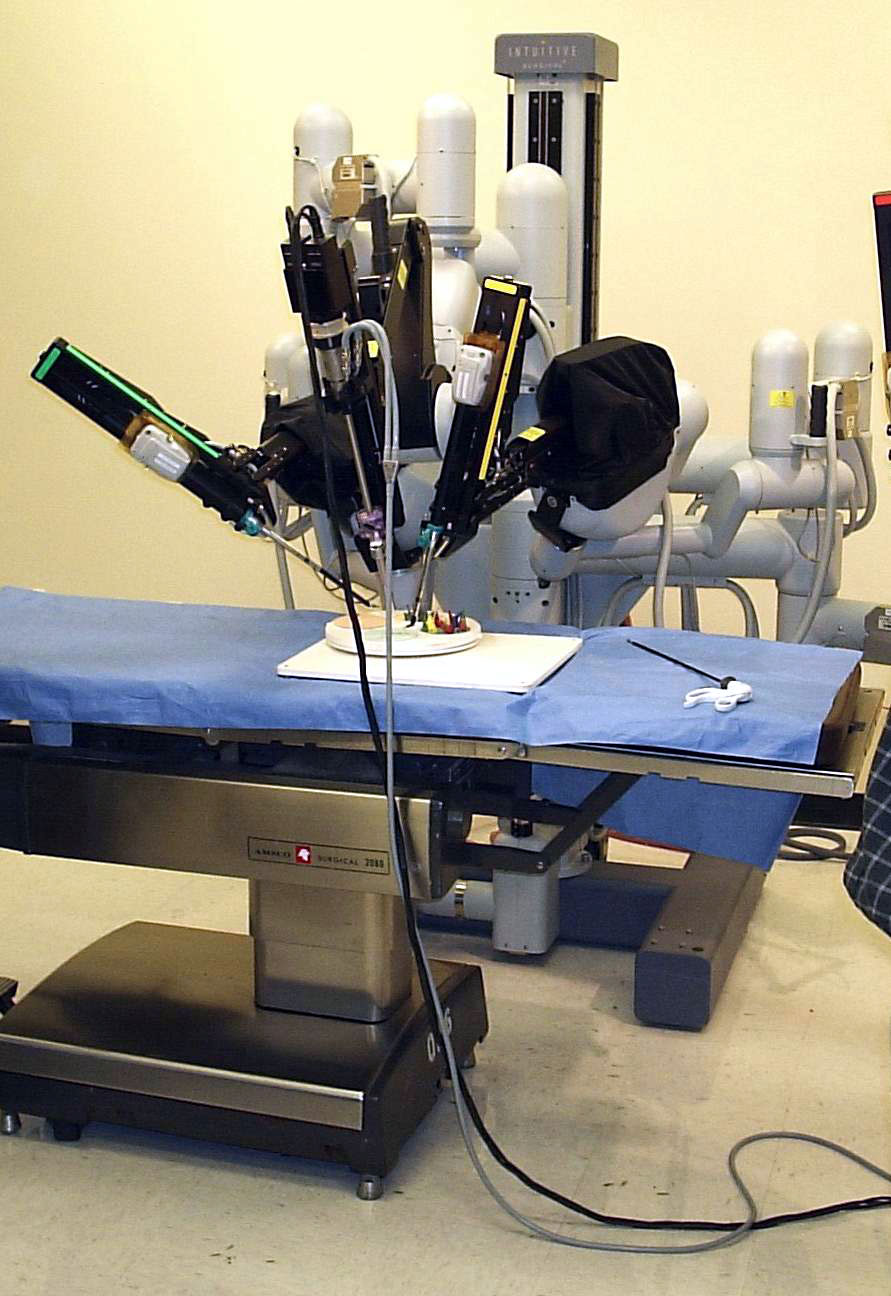
\includegraphics[scale=0.07]{./EtapaModerna/Imagenes/robot_surgery.jpg}
		\caption{Robot para laparoscopia \href{https://es.m.wikipedia.org/wiki/Archivo:Laproscopic_Surgery_Robot.jpg}{Wikimedia, por Nimur}}
	\end{subfigure}
\end{figure}
\end{frame}

%%%%%%%%%%%%%%%%%%%%%%%%%%%%%%%%%%%%%%%%%%%%%%%%%%%%%%%%%%%%%%%%%%%%%%%%%%%%%%%%%%%%%%%%%%%%%%
%%                                    Robots Humanoides                                     %%
%%%%%%%%%%%%%%%%%%%%%%%%%%%%%%%%%%%%%%%%%%%%%%%%%%%%%%%%%%%%%%%%%%%%%%%%%%%%%%%%%%%%%%%%%%%%%%

\begin{frame}[fragile]{Robots Humanoides}
\vspace{10px}
\pause
\metroset{block=fill}
\begin{block}{Principales Robots}
	\begin{itemize}
		\item Actroid: asistente por voz sencillo. \href{https://www.youtube.com/watch?v=p-8GEcLRRAM}{(Vídeo)}
		\pause
		\item Wakamaru: robot para las casas. \href{https://www.youtube.com/watch?v=k6zB-HDtI_0}{(Vídeo)}
		\pause
		\item iCub: imitación de movimientos humanos complejos. \href{https://www.youtube.com/watch?v=ZcTwO2dpX8A}{(Vídeo)}
		\pause
		\item Sophia: interacción oral y gestual. Gestión de las emociones. \href{https://www.youtube.com/watch?v=S5t6K9iwcdw}{(Vídeo)}
	\end{itemize}
\end{block}
\begin{figure}
	\centering
	\pause
	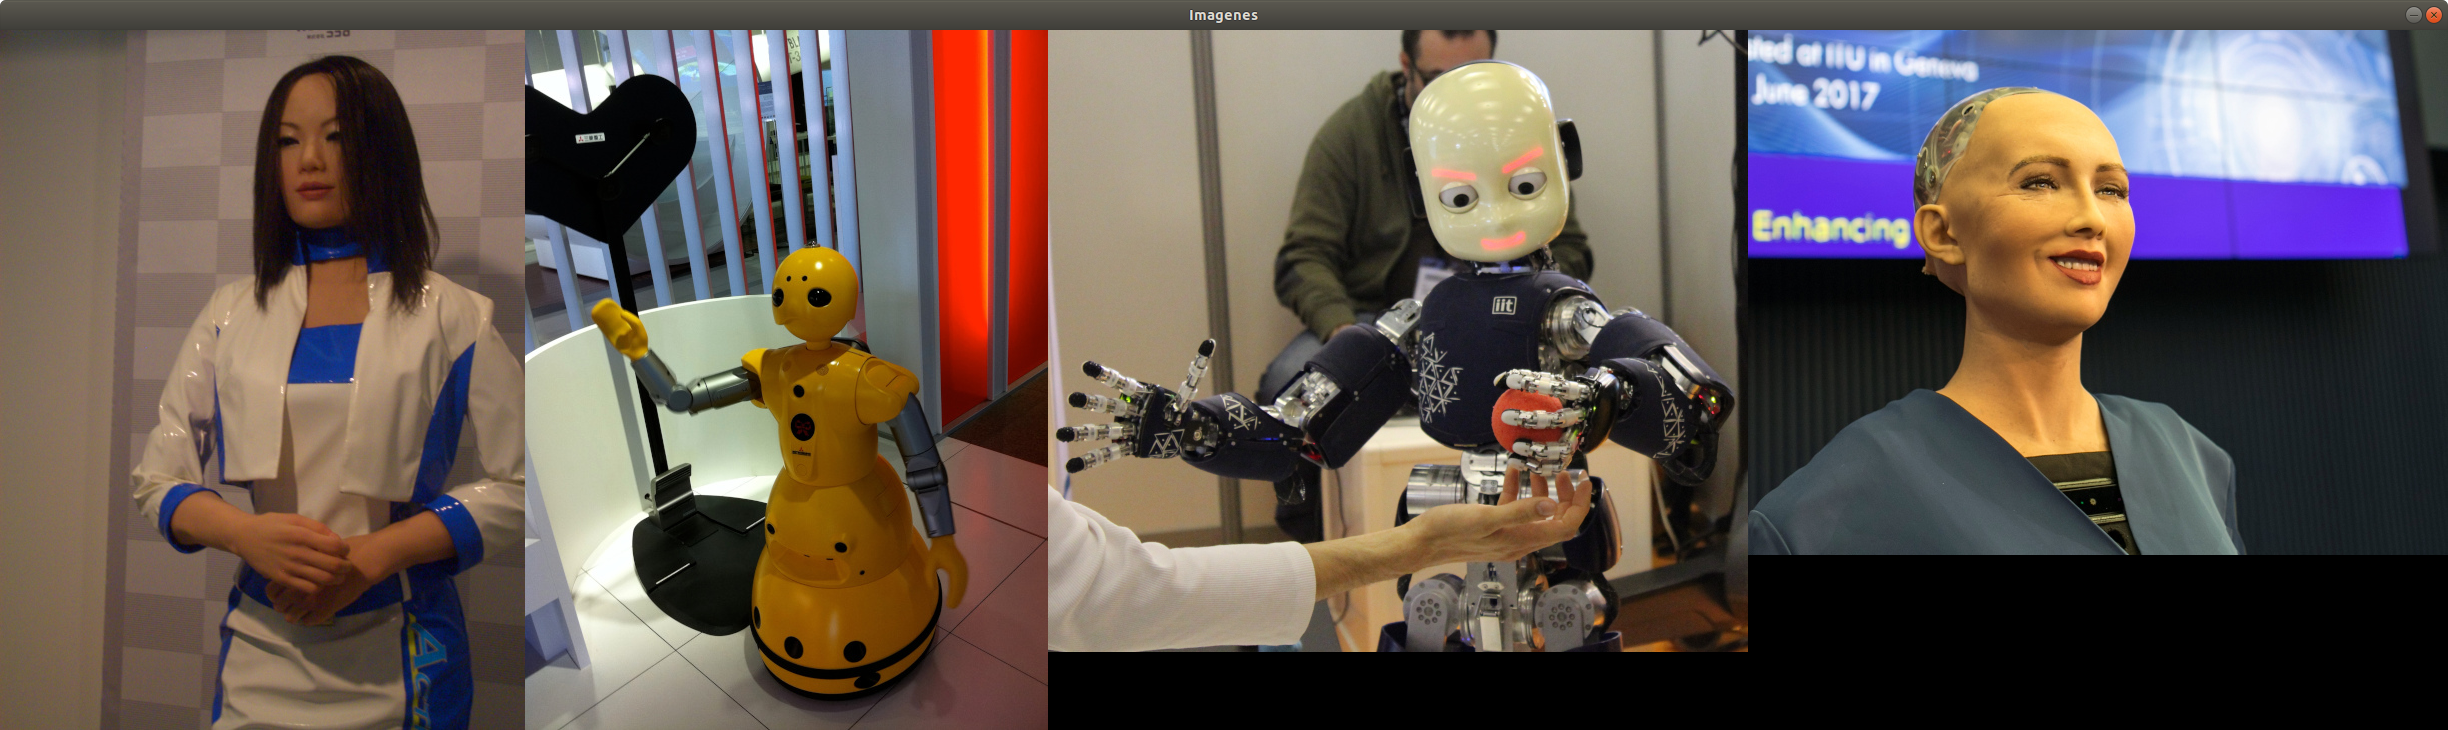
\includegraphics[scale=0.12]{./EtapaModerna/Imagenes/robots_humanoides.png}
	\caption{Actroid \href{https://commons.wikimedia.org/wiki/File:Actroid_3.jpg}{Wikimedia}, Wakamaru \href{https://commons.wikimedia.org/wiki/File:Wakamaru-fullshot2011.jpg}{Wikimedia}, iCub \href{https://commons.wikimedia.org/wiki/File:ICub_Innorobo_Lyon_2014.JPG}{Wikimedia}, Sophia \href{https://es.wikipedia.org/wiki/Archivo:Sophia_(robot).jpg}{Wikimedia}}
\end{figure}
\end{frame}



\end{document}
